\documentclass[review]{siamart220329}
\setlength{\emergencystretch}{3em}
% siamart220329 already loads hyperref, xcolor, algorithm (float), graphicx is NOT loaded
\usepackage{amsmath,amssymb,booktabs,graphicx,enumitem,float}
\usepackage{algpseudocode}
\newcommand{\Om}{\mathcal{O}(m)}
\newcommand{\R}{\mathbb{R}}
\hypersetup{colorlinks=true,allcolors=blue!55!black}

\title{NLF: A Resistor-Network Framework and Linear-Time Solver for Convex Network-Flow Equilibria\thanks{Submitted to the editors \today.}}
\author{Oren E. Livne\thanks{Pine Birch Analytics, 35 Kelinger Rd, Churchville, PA 18966-1033 (\texttt{oren.livne@gmail.com}, tel.\ 312-533-9130, \texttt{pinebirchanalytics.com}; ORCID: \href{https://orcid.org/0000-0001-6700-483X}{0000-0001-6700-483X}).}}
\headers{NLF: a linear-time solver for network-flow equilibria}{O. E. Livne}

\begin{document}
\maketitle

\begin{abstract}
We present \textbf{NLF} (Nonlinear Laplacian Flow), a unified framework and linear-time solver for
convex network-flow equilibria. A broad class of flow problems---congestion (traffic) routing,
minimum-delay communication routing, and maximum flow---is the stationarity of a convex,
edge-separable energy and shares one form: a \emph{nonlinear graph Laplacian}
$B\,\rho(B^{\top}\phi)=\alpha d$, in which a single monotone edge law $\rho_e$ encodes the physics.
All problems are posed in \emph{undirected} form: flows are signed, each edge law is odd, and
capacities---maximum flow included---bound the flow magnitude in either orientation; directed,
arc-based variants are future work. The energy is classical---the optimality system of a convex, edge-separable network-flow program
(monotropic programming); what is new is the \emph{unification}, that one monotone edge law
parametrizes all three problems, together with how it is solved: where electrical-flow
and interior-point methods for flow drive an \emph{outer} reweighting or barrier loop around
\emph{linear} Laplacian solves to reach an \emph{approximate} optimum, NLF puts the nonlinearity
in the edge law itself, so one energy encodes the problem \emph{exactly}. NLF solves it by a damped
chord-Newton iteration whose frozen global linearization---itself a weighted graph Laplacian---is
inverted by a lazily refreshed near-linear Laplacian solver applied directly to the nonlinear
residual; the framework is engine-agnostic (we use LAMG+, and verify approximate Cholesky is
interchangeable). Each inner solve is $\Om$ and the whole nonlinear solve costs $2$--$4$ linear
Laplacian solves (up to $\sim$7 on the largest social graphs). On \emph{undirected, single-commodity}
congestion over real road-network topologies
(BPR cost) NLF matches a state-of-the-art interior-point method \emph{on the identical convex program}
to $10^{-10}$, in a step count with no size trend, at empirically near-linear cost; on poorly-separable
graphs---where the IPM's direct KKT core is superlinear---the speed-up over that interior-point baseline
widens past $45\times$ (synthetic Erd\H{o}s--R\'enyi graphs, an extreme low-separability case). The
inner solve is a replaceable module---a matrix-free first-order method on the dual ties NLF on
\emph{well-conditioned} graphs---but multigrid is the robust default: running all three paradigms
(multigrid-Newton, interior-point, first-order) on the same program across $1{,}669$ SuiteSparse
graphs, \emph{NLF converges on every one}, is fastest-or-only on $85\%$ (median $2.6\times$/$4.2\times$
faster than the interior-point/first-order baselines where they converge), and is the \emph{only}
solver to finish within the time budget on the $90$ hardest graphs---ill-conditioned and
poorly-separable at once (first-order slowed by the former, sparse-direct by the latter).
Robustness is broad: across the full SuiteSparse collection ($2{,}003$ graphs to $1.8\times10^7$ edges,
plus giants to $5.6\times10^7$), under one BPR instance per graph, NLF converged on all of them at a
median of $18$ cycles, with a fitted time exponent $t\propto m^{0.98}$. A
first multicommodity extension routes $K$ commodities through one shared hierarchy at $\mathcal{O}(Km)$
per step---corpus-wide at $K=4$ ($3.8\times$ single-commodity cost)---and yields a measured finding:
on real capacity data, congestion couples commodities by inflating shared-corridor costs (up to
$8.8\times$), not by rerouting them. The same machinery recovers the exact combinatorial max-flow as
a short sequence of Laplacian solves, with the cut potential as a by-product.
\end{abstract}

\begin{keywords}
network equilibrium, traffic assignment, maximum flow, algebraic
multigrid, nonlinear multigrid, inexact Newton methods, continuation, graph Laplacian
\end{keywords}

\begin{AMS}
90B20, 90C35, 65F10, 65N55, 90B10, 05C21
\end{AMS}

\section{Introduction}\label{sec:intro}
Flows on networks at equilibrium are everywhere: drivers distributing over a road map until no route
is faster (traffic assignment~\cite{beckmann,bpr,boyles-tna}), packets routed to minimize delay in a
communication network~\cite{bertsekas-gallager,mendiola-te}, current in a resistor
network~\cite{doyle-snell}, and---at the combinatorial extreme---the maximum flow through a
capacitated graph~\cite{ahuja-magnanti-orlin,goldberg-tarjan,chen-almost-linear}. These look like different problems with different algorithms: traffic assignment is solved by
Frank--Wolfe or general convex optimization, max-flow by augmenting-path or push--relabel
combinatorics. We make a unifying observation and build a single fast solver on it.

\paragraph{The observation} Each of these is the stationary point of a convex, edge-separable
energy in the node potentials, and its Euler equation is one and the same \emph{nonlinear graph
Laplacian},
\begin{equation}\label{eq:master}
B\,\rho(B^{\top}\phi)=\alpha\,d ,
\end{equation}
where $B$ is the node--edge incidence matrix, $\phi$ the node potentials, $d$ a source/sink demand,
$\alpha$ a load, and $\rho_e$ a \emph{monotone edge law} that alone encodes the physics: a
saturating $\rho_e$ gives a hard capacity (max flow); a gently rising $\rho_e$ gives a congestion
cost (traffic). The flow is $f_e=\rho_e\big((B^{\top}\phi)_e\big)$, and every Newton linearization of
\eqref{eq:master} is an ordinary weighted graph Laplacian $J=B\,\mathrm{diag}(\rho')B^{\top}$. A fast
\emph{near-linear} graph-Laplacian solver therefore solves all of them. What makes the
\emph{nonlinear} problem cheap is not which solver that is, but how it is used: a single global
linearization---itself a weighted graph Laplacian---is frozen across steps, lazily refreshed, and
inverted directly against the nonlinear residual as a damped, inexact chord-Newton iteration, rather
than solved to a tolerance of its own, with the continuation woven into the same loop; the entire
nonlinear solve costs $2$--$4$ linear Laplacian solves (\S\ref{sec:accuracy}). Any near-linear
Laplacian solver serves as this inner engine---the framework is engine-agnostic
(\S\ref{sec:inner})---and we use \textbf{LAMG+}~\cite{lamgplus}, a lean algebraic multigrid solver
robust across graph classes, as a convenient parameter-free default, having verified that approximate
Cholesky is fully interchangeable. One incidental convenience of LAMG+'s affinity-based aggregation is
that it naturally respects the saturating min cut, though the framework does not depend on it
(\S\ref{sec:inner}).

\subsection{Contribution}\label{sec:contrib}
This paper makes three contributions, in order of practical weight.
\begin{enumerate}[leftmargin=1.6em,itemsep=1pt]
\item \emph{A unifying resistor-network formulation} (\S\ref{sec:formulation}) that casts maximum
flow, congestion (traffic) routing, and minimum-delay routing as one nonlinear Laplacian
\eqref{eq:master}, with the problem class fixed by a single monotone edge law and the easy/hard
dichotomy (no-fold vs.\ fold; \S\ref{sec:formulation}) fixed by whether that law saturates. The stationarity equation itself
is classical---it is the optimality system of a convex, edge-separable network-flow program (monotropic
programming); our contribution is the \emph{unification}, that one edge law parametrizes all three
problems, together with its operational consequence: a \emph{single solver} addresses the whole class.
Unlike the electrical-flow and interior-point ``Laplacian paradigm'' for flow~\cite{christiano-etal,daitch-spielman},
which drive an outer reweighting/barrier loop around \emph{linear} solves to an $(1+\epsilon)$-approximate
optimum, here the nonlinearity sits in the edge law and the equilibrium reached is \emph{exact}.
\item \emph{A linear-time solver for convex congestion flow} (\S\ref{sec:traffic})---establishing
the two claims on which any larger congestion solver rests: that the convex Beckmann equilibrium is
exactly \eqref{eq:master}, and that a robust $\Om$ near-linear Laplacian inner solve makes it
linear-time. No combinatorial algorithm addresses this problem. NLF matches a state-of-the-art IPM
to $10^{-10}$ in a flat step count; on poorly-separable graphs NLF is the only $\Om$ solver and wins
past $45\times$ (\S\ref{sec:bprscale}). Robustness is corpus-wide: $2{,}003$ SuiteSparse graphs
converge, $t\propto m^{0.98}$, entire nonlinear solve $2$--$4$ linear solves
(\S\ref{sec:corpus},~\ref{sec:accuracy}). A first multicommodity layer (\S\ref{sec:mc}) carries $K$
commodities through one hierarchy at $\mathcal{O}(Km)$; on real capacity data coupling inflates
shared-corridor costs (${\le}8.8\times$) without rerouting.
\item \emph{An $\Om$ maximum-flow solver} (\S\ref{sec:maxflow}). The saturating instance recovers the
\emph{exact} combinatorial max-flow as a short, size-independent sequence of Laplacian solves, with
the cut respecting multigrid coarsening arising for free. Not faster than a tuned combinatorial solver,
but returns the cut potential and full parametric flow curve.
\end{enumerate}
Extensions---directed multicommodity assignment and a full-multigrid variant---are outlined in
\S\ref{sec:extensions}.

\subsection{The practical problem and its applications}\label{sec:applications}
Computing an equilibrium flow on a large network is a recurring industrial task, and in each domain
the computational bottleneck is the same Laplacian-structured solve at the core of \eqref{eq:master}.

\emph{Road traffic (assignment).} Metropolitan planning agencies compute user-equilibrium traffic
assignment---how drivers distribute over a road map until no route is faster---to evaluate road
projects and pricing~\cite{beckmann,bpr,boyles-tna}. This is the convex Beckmann program with the
BPR congestion law; it is NLF's no-fold instance and the setting of our sharpest result
(\S\ref{sec:traffic}). The incumbent solvers are Frank--Wolfe and bush-based methods
(\S\ref{sec:competitor}).

\emph{Communication and data-center routing (minimum delay).} Routing packets to minimize end-to-end
delay under the Kleinrock $M/M/1$ model~\cite{bertsekas-gallager,mendiola-te} is the same equilibrium
with a capacity-saturating delay law---a fold instance handled by the continuation of
\S\ref{sec:continuation}.

\emph{Maximum flow (logistics, scheduling, vision).} The capacitated maximum-flow problem
\cite{ahuja-magnanti-orlin,goldberg-tarjan} is the saturating-law extreme of the same energy
(\S\ref{sec:maxflow}); NLF recovers the exact value together with the min cut and the full
flow-vs-load curve. Combinatorial solvers are faster on the bare value, but do not return the smooth
interior flow or the parametric curve that an outer optimizer manipulates when max flow is an inner
step.

\emph{Nonlinear resistor and analog-circuit networks.} The most literal instance: monotone
two-terminal devices (diodes, varistors, memristors) in DC steady state give \eqref{eq:master} with
$\rho_e$ the device $I$--$V$ law---the form of DC circuit analysis and in-memory-computing crossbars.
As with OPF (\S\ref{sec:outofscope}) these topologies are typically structured (direct's regime); the
edge would appear only on large, irregular analog networks.

Across all of these the operator wants not a one-off number but the equilibrium, its
binding-constraint structure, and its sensitivity to load, at a scale where the linear-algebra cost
dominates---the gap NLF targets.

\subsubsection{Out of scope: power-grid optimal power flow}\label{sec:outofscope}
One natural-looking application is \emph{not} an NLF win, and we state so up front. In the widely used
DC approximation, optimal power flow (OPF) with transmission \emph{line limits} is exactly a
capacity-constrained flow on the grid graph: the power balance $B'\theta=p$ is a susceptance-weighted
graph Laplacian, the line limits are the box constraints of the saturating law \eqref{eq:rho}, and
the dispatch is set by the binding lines (a min cut) and their shadow prices (locational marginal
prices)---objects NLF returns. The mapping is exact, and continental, contingency-constrained OPF is
an active, funded need~\cite{matpower,powermodels,arpae-go}. \emph{But} transmission grids are
well-separated (near-planar), the regime where sparse-direct factorization of the same Laplacian is
near-optimal: on the real grids we tested ($118$ to $30{,}000$ buses, plus the power-flow/OPF matrices
embedded in SuiteSparse) direct is \emph{faster} than NLF by $2$--$5\times$, widening to $6\times$ on
a $10{,}000$-bus system (\S\ref{sec:vsdirect}). \textbf{NLF is therefore not a faster DC-OPF solver,
and we make no such claim;} we record DC-OPF as a conceptual instance, not a performance result.
Full \emph{AC} OPF is further out of reach: non-convex, with a non-Laplacian power-flow Jacobian,
outside the convex monotone-edge-law class this paper addresses
entirely.

\subsection{Prior work, and how NLF differs}\label{sec:priorwork}
Three lines of work meet at \eqref{eq:master}; NLF sits in the gap none of them fills.

\emph{The Laplacian paradigm for flow.} Electrical-flow algorithms~\cite{christiano-etal} and
interior-point methods for generalized flow~\cite{daitch-spielman} solve a \emph{sequence of linear}
weighted-Laplacian systems inside an outer multiplicative-weights or barrier loop, reaching a
$(1+\epsilon)$-approximate optimum; the flow is a \emph{linear} function of the potential and all
nonlinearity lives in the outer schedule. NLF instead places the nonlinearity in the constitutive
law $f=\rho(B^{\top}\phi)$, so a single energy encodes the capacity \emph{exactly} and the
equilibrium reached is exact, not $(1+\epsilon)$ (\S\ref{sec:formulation}).

\emph{Fast linear Laplacian solvers.} Nearly-linear solvers for $Lx=b$---combinatorial
multigrid~\cite{koutis-cmg}, support-tree/Spielman--Teng theory~\cite{spielman-teng}, approximate
Cholesky~\cite{approxchol,gks2023}, and algebraic multigrid including
LAMG~\cite{lamg}---address the \emph{linear, unconstrained} problem only. They are the engine, not
the method: NLF calls a robust $\Om$ linear solver (LAMG+) as its inner kernel but adds the
nonlinear, capacity-constrained equilibrium layer on top. AMG has also been applied to the
\emph{square, unconstrained} power-flow \emph{equations}~\cite{bindel-amg-pf}; that is a different
problem class (no objective, no inequality constraints) from the constrained flow program here.

\emph{Multilevel optimization.} NLF is \emph{not} multilevel optimization in the MG/OPT
sense~\cite{nash-mgopt,gratton-rmtr}: it does not build coarse \emph{optimization} models or recurse
the objective. It reduces the equilibrium to a \emph{single} nonlinear equation \eqref{eq:master} and
uses multigrid only as the \emph{linear} inner solve inside a frozen-linearization chord-Newton
continuation; the nonlinearity is carried by the edge law and the outer continuation, not by a
coarse-grid objective.

\emph{Combinatorial and transport-specific solvers.} Augmenting-path and push--relabel max-flow
\cite{goldberg-tarjan,boykov-kolmogorov} and the almost-linear-time exact algorithm
\cite{chen-almost-linear} target directed max/min-cost flow; Frank--Wolfe~\cite{frankwolfe} and
bush-based assignment (Algorithm~B~\cite{bargera2002}, TAPAS~\cite{bargera2010}) target the
smooth-cost traffic program. Each is specialized to one problem class. NLF's contribution is
orthogonal: a \emph{single} solver, parametrized by one edge law, that spans all of them and inherits
graph-class robustness from its multigrid core. We benchmark against representatives of each family
where a runnable one exists (Frank--Wolfe and Ipopt~\cite{ipopt} for congestion, Boykov--Kolmogorov
for max flow) and position the rest honestly where it does not (\S\ref{sec:competitor}).

\section{A unified resistor-network formulation}\label{sec:formulation}
Let $B$ be the $n\times m$ node--edge incidence matrix of a connected graph, $\phi\in\R^n$ node
potentials, $d$ a demand with $\mathbf 1^{\top}d=0$, and $\alpha\ge0$ a load. Give each edge a smooth,
strictly convex \emph{co-potential} $\Psi_e$ and let its derivative be the edge law
\begin{equation}\label{eq:law}
f_e=\rho_e(g_e),\quad \rho_e=\Psi_e',\quad g_e=(B^{\top}\phi)_e ,
\end{equation}
a monotone map from potential gradient to flow. Equilibrium is the stationary point of the convex
energy $E(\phi)=\sum_e\Psi_e\big((B^{\top}\phi)_e\big)-\alpha\,d^{\top}\phi$, i.e.\ \eqref{eq:master}.
Equivalently, in flow variables it is the convex program
\begin{equation}\label{eq:primal}
\min_f\ \sum_e\Phi_e(f_e)\quad\text{s.t.}\quad Bf=\alpha d ,\qquad \Phi_e=\Psi_e^{*}\ \text{(Legendre dual)},
\end{equation}
whose multipliers are the potentials $\phi$; the marginal cost is $t_e=\Phi_e'=\rho_e^{-1}$.
The Newton linearization of \eqref{eq:master} is the weighted graph Laplacian
\begin{equation}\label{eq:jac}
J=B\,\mathrm{diag}\!\big(\rho'(B^{\top}\phi)\big)\,B^{\top},\qquad
w_e=\rho'_e(g_e)=\Psi_e''(g_e)=1/t_e'(f_e)\ge0 ,
\end{equation}
a \emph{solution-dependent conductance network}. Everything specific to a problem lives in the one
scalar law $\rho_e$; the solver below never sees anything but $\rho_e,\rho'_e$ and $J$.
Appendix~\ref{app:instances} derives, for each application in turn, the equilibrium principle, the
convex program it is equivalent to, and the reduction of its KKT system to \eqref{eq:master}---in
particular, where the complementarity conditions of the directed problems go.

\paragraph{The fold dichotomy} The single feature that governs difficulty is whether the edge law
\emph{saturates}. Table~\ref{tab:instances} lists three standard instances.
\begin{itemize}[leftmargin=1.4em,itemsep=1pt]
\item \emph{Hard capacity (saturating $\rho$, conductance $\to0$).} The flow cannot exceed a capacity
$c_e$, so $\rho_e$ is bounded and $\rho'_e\to0$ as the edge saturates. As the load rises to a
\emph{feasibility limit}, the saturating edges form a cut and $J$ \emph{folds}---a continuation
turning (limit) point where $\alpha$ caps at the min cut $F^*$ and $J$ becomes singular. Maximum flow ($\rho_e=c_e\tanh(g/c_e)$) and minimum-delay communication routing
(Kleinrock delay $t_e(f)=1/(c_e-f)$, capacity $c_e$) are of this type; they need continuation through
the fold (\S\ref{sec:continuation}).
\item \emph{Soft congestion (rising $\rho$, conductance bounded).} The cost rises with flow but
imposes no hard cap, so $\rho_e$ is unbounded and $\rho'_e$ stays in $(0,\rho'_{\max}]$, bounded away
from $0$: there is \emph{no} feasibility limit and \emph{no} fold. Traffic assignment with the BPR
cost is of this type; $J$ is uniformly well-conditioned and NLF needs no continuation (\S\ref{sec:traffic}).
\end{itemize}

\begin{table}[t]\centering\small
\caption{Three instances of the resistor-network framework \eqref{eq:master}. The edge law $\rho_e$
(flow vs.\ potential gradient) is the inverse of the marginal cost $t_e=\Phi_e'$. ``Fold'' marks a
feasibility limit where the conductance $\rho'_e\to0$ and $J$ becomes singular.}\label{tab:instances}
\resizebox{\columnwidth}{!}{%
\begin{tabular}{lllcl}
\toprule
Problem & Marginal cost $t_e(f)$ & Conductance $\rho'_e$ & Fold? & Application\\
\midrule
maximum flow~\cite{ahuja-magnanti-orlin,goldberg-tarjan-cacm} & box $|f|\le c_e$ (soft barrier) & $\to0$ at cut      & yes & vision, matching\\
min-delay routing~\cite{bertsekas-gallager,mendiola-te} & $1/(c_e-f)$ (Kleinrock)         & $\to0$ at $f\!\to\!c_e$ & yes & communication\\
congestion~\cite{beckmann,bpr,boyles-tna}  & $t^0_e\big(1+b(f/c_e)^{p}\big)$  & $\in(0,\rho'_{\max}]$ & no  & road traffic\\
\bottomrule
\end{tabular}}
\end{table}

\paragraph{The max-flow law in detail} For the saturating instance used in \S\ref{sec:maxflow},
take
\begin{equation}\label{eq:rho}
\rho_e(g)=\begin{cases} c^+_e\tanh(g/c^+_e), & g\ge0,\\[2pt]
-c^-_e\tanh(g/c^-_e), & g<0,\end{cases}
\qquad
\Psi_e(g)=c_e^{2}\log\cosh(g/c_e),
\end{equation}
a soft-capacity barrier: $\Psi_e(g)=\tfrac12 g^2$ for $|g|\ll c_e$ (a unit resistor) and grows only
linearly, $\Psi_e\to c_e|g|$, for $|g|\gg c_e$ (a saturated edge), so $\rho_e=\Psi_e'$ clamps the flow
smoothly to $-c^-_e\le f_e\le c^+_e$. Here $w_e=1-(f_e/c_e)^2\in[0,1]$ is a pure ``edge openness,''
$1$ for a slack edge and $0$ for a saturated one, and \textbf{the forming min-cut is exactly the
zero-conductance set}---which is why algebraic-multigrid aggregation, driven by a relaxation-based
strong-connection measure, refuses to coarsen across it (\S\ref{sec:maxflow}). The congestion (BPR)
law is given where it is used, in \S\ref{sec:traffic}.

\begin{figure}[t]\centering
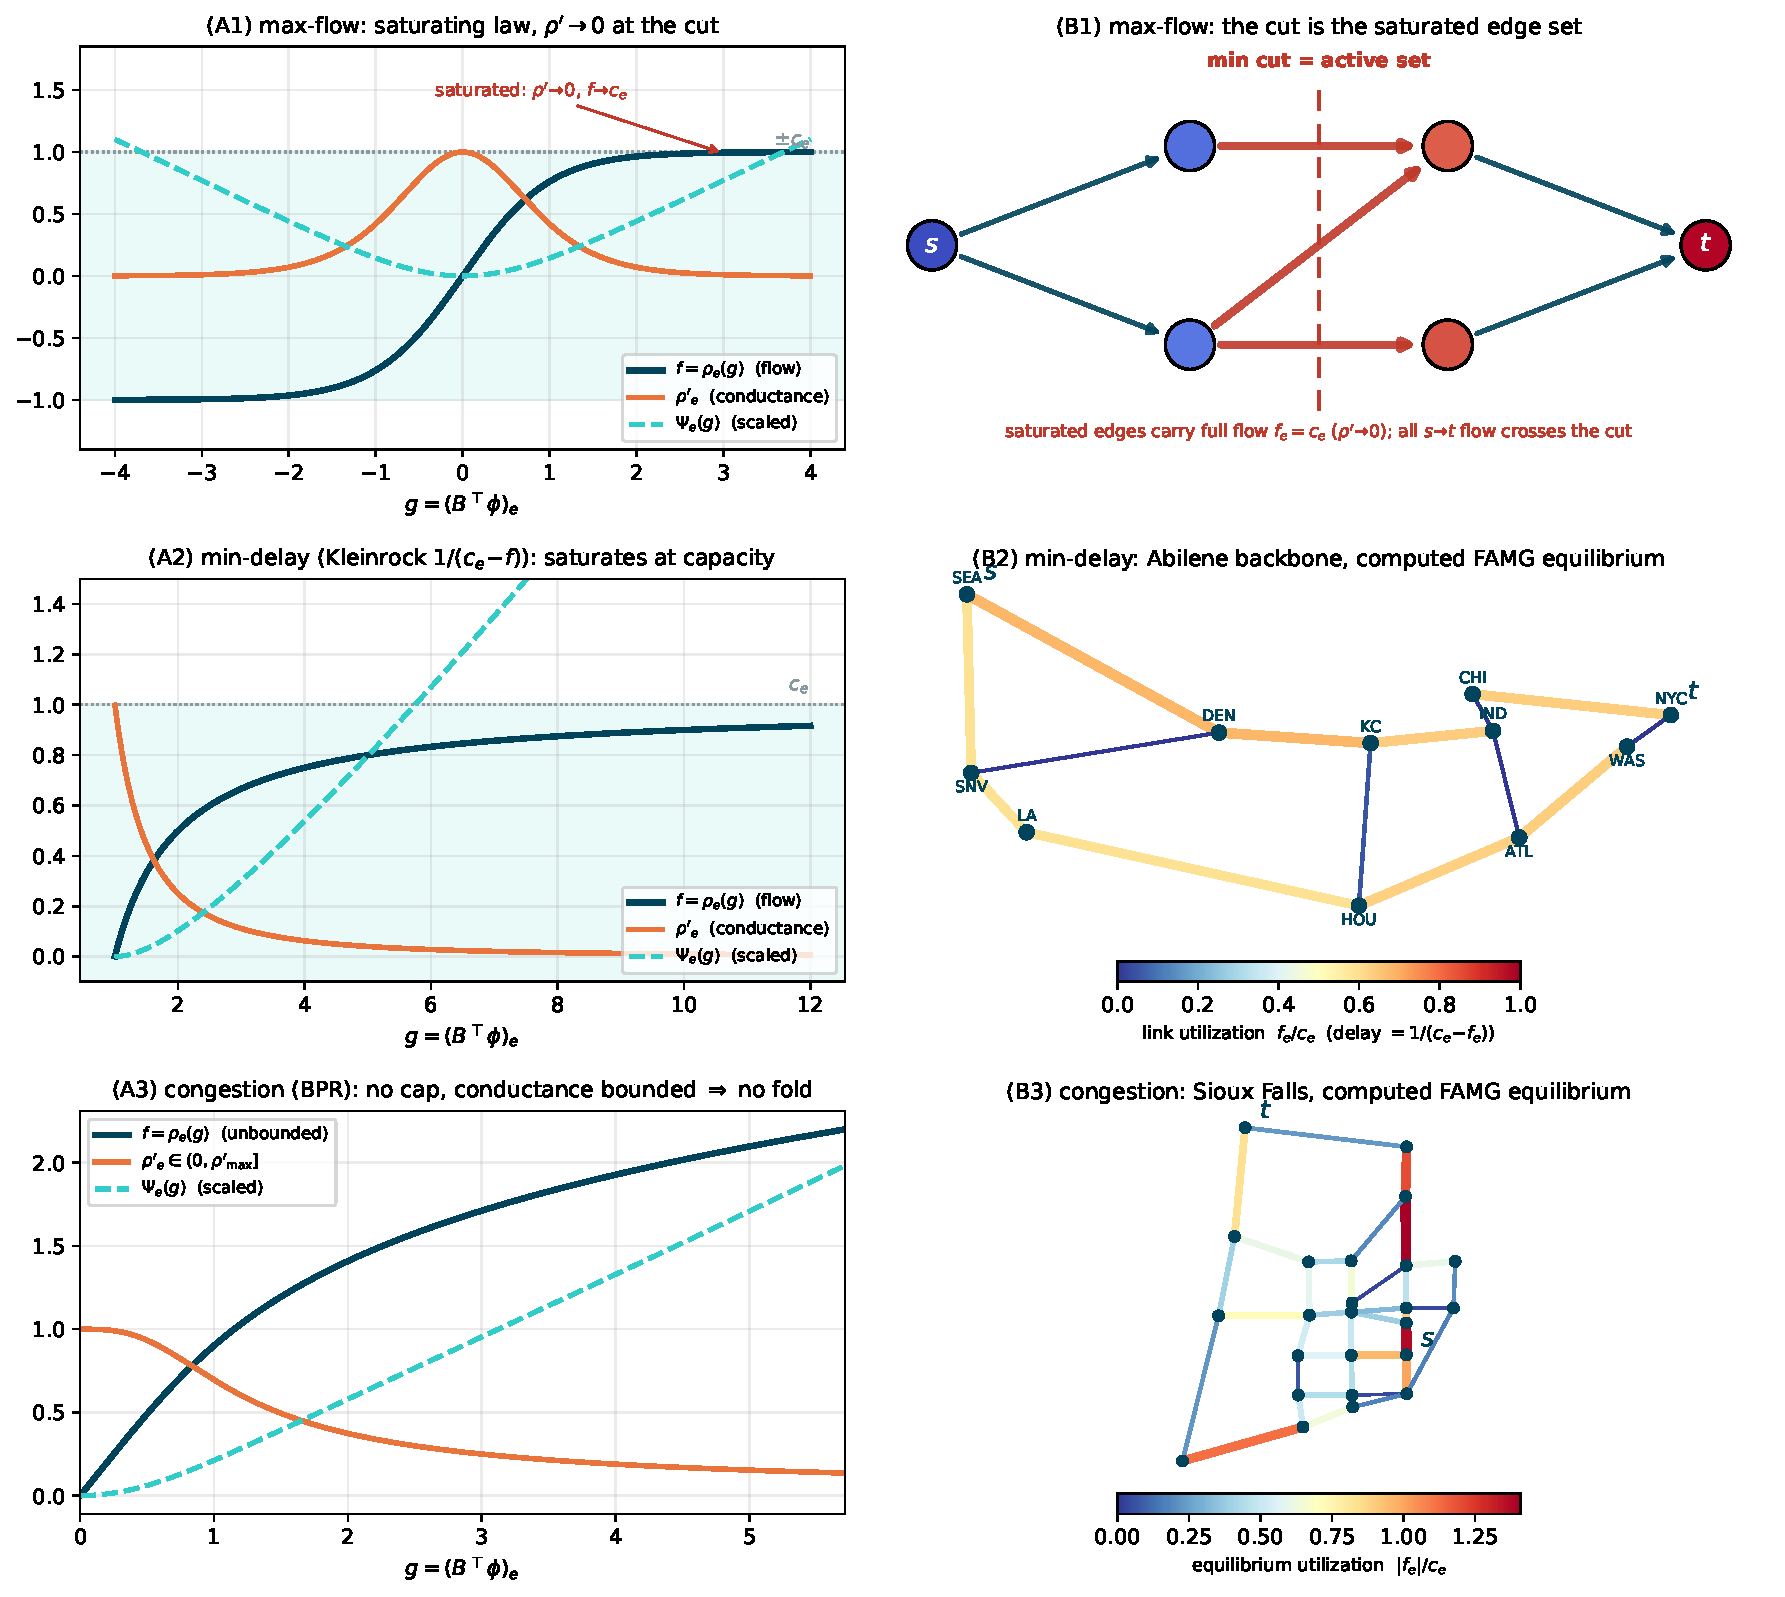
\includegraphics[width=\textwidth]{nlf_formulation.pdf}
\caption{The three instances of the framework (one row per line of Table~\ref{tab:instances});
column (A) the edge law $\rho_e$ (flow), its derivative $\rho'_e$ (the solution-dependent
conductance) and the energy $\Psi_e$; column (B) the behavior it induces.
\emph{Row 1, max-flow (tanh):} the law saturates at $\pm c_e$ and $\rho'_e\to0$; (B1) the saturated
edges are the min cut = the active set, and $\phi$ steps across them.
\emph{Row 2, minimum-delay routing (Kleinrock $1/(c_e\!-\!f)$):} the law saturates at capacity---the
fold class, handled by the continuation of \S\ref{sec:continuation}; (B2) the real application: the
Abilene/Internet2 backbone colored by the \emph{computed} NLF min-delay equilibrium for a
Seattle$\to$New York demand.
\emph{Row 3, congestion (BPR):} the law is unbounded and $\rho'_e$ is bounded away from zero---no
fold, pure cycling; (B3) the real application: the Sioux Falls road network colored by the
\emph{computed} NLF equilibrium utilization $|f_e|/c_e$ for a single source--sink demand
(\S\ref{sec:traffic}).}\label{fig:form}
\end{figure}

\paragraph{Relation to prior Laplacian-paradigm formulations} Solving flow through graph-Laplacian
systems is the core of a productive line of work, but NLF's mechanism differs in a way that is the
source of its novelty. Electrical-flow methods~\cite{christiano-etal} and their $p$-Laplacian
descendants compute a sequence of \emph{linear} electrical flows $f=\mathrm{diag}(w)\,B^{\top}\phi$
---each a fixed weighted-Laplacian solve---and steer an \emph{outer} multiplicative-weights loop to a
$(1+\epsilon)$-approximate max-flow; interior-point methods for (generalized) flow
\cite{daitch-spielman} likewise wrap a Laplacian solve in a barrier path-following loop. In both, the
flow is a \emph{linear} function of the potential and all nonlinearity lives in the outer schedule.
NLF instead places the nonlinearity in the \emph{constitutive law}: $f=\rho(B^{\top}\phi)$ is a
nonlinear, saturating function of the gradient, so the single energy of \eqref{eq:master} encodes the
capacity \emph{exactly} and its feasibility limit is the \emph{exact} min cut, not a $(1+\epsilon)$
relaxation; the outer loop is then a short continuation through one scalar fold, not a reweighting or
barrier schedule. The Beckmann congestion instance \eqref{eq:primal} is itself classical
\cite{beckmann}; what is new is the saturating-resistor reformulation of max-flow and the unified
monotone-edge-law family that places max-flow, congestion, and minimum-delay routing under one
nonlinear Laplacian, each solved by the same algebraic-multigrid inner solve.

\section{The NLF algorithm}\label{sec:algorithm}
NLF is a \emph{continuation loop over the load} $\alpha$. Each fixed-$\alpha$ subproblem is solved
by a handful of multigrid cycles applied \emph{directly to the nonlinear residual}: a LAMG+
hierarchy, built once from the linearization $J=B\,\mathrm{diag}(\rho')B^{\top}$ \eqref{eq:jac} at
some earlier iterate and \emph{frozen} across steps, is cycled against
$-r(\phi)=\alpha d-B\rho(B^{\top}\phi)$, and the resulting correction is accepted through a line
search. In classical terms this is a \emph{damped, inexact chord-Newton iteration}: a global
linearization, frozen---operator and hierarchy alike---across steps and re-formed only when an
observed-convergence monitor says it has drifted too far, its inverse applied by $\Om$ multigrid
cycles rather than by an inner solve to a tolerance of its own. We
present the algorithm from its simplest component to its most complex: the linear engine
(\S\ref{sec:inner}), the fixed-load solve (\S\ref{sec:fas}), and the continuation through the fold
(\S\ref{sec:continuation}). Three principles organize the design.
\begin{enumerate}[leftmargin=1.6em,itemsep=1pt]
\item \emph{Reuse the linear engine.} Every linearization of \eqref{eq:master} is an ordinary
weighted graph Laplacian, so the cycle is a lean algebraic multigrid solver run on $J$, unchanged.
\item \emph{Freeze the hierarchy (lazy-setup reuse).} Across a chain of nearby linearizations the AMG
hierarchy is reused rather than rebuilt---an operator-reuse / lazy-setup strategy (distinct from
Brandt's frozen-$\tau$, which freezes the FAS coarse-grid $\tau$ correction, a right-hand-side
quantity~\cite[\S15]{brandt-guide}): touch the setup rarely, and let an observed-convergence monitor
decide when the frozen levels have drifted too far.
\item \emph{Continue only through folds.} Where the law saturates, $\alpha$ folds at the feasibility
limit; the well-conditioned continuation variable is the cut-mode amplitude. Where it does not, no
continuation is needed.
\end{enumerate}

\subsection{The inner Laplacian solve}\label{sec:inner}
The outer loop requires only a near-linear solver for graph Laplacians; the framework is agnostic to
which one. We use LAMG+ as a convenient, parameter-free default. LAMG+ is a lean caliber-1 aggregation algebraic multigrid solver for graph Laplacians: it aggregates
nodes by a relaxation-based affinity, bounds the coarse-operator energy by a guard rather than an
aggregate-size cap, eliminates low-degree nodes by exact Schur complements, and accelerates a
fractional cycle by min-residual iterate recombination. The companion paper~\cite{lamgplus}
establishes its two properties we rely on: it solves $L\phi=b$ in
$\mathcal{O}(m\log(1/\varepsilon))$ work with \emph{no parameter tuning} across $1{,}374$ real-world
graphs of every class, and on the large poorly-separable graphs---where sparse direct methods
exhaust memory---it is among the fastest solvers available. The leading alternative near-linear
graph-Laplacian solvers---approximate Cholesky \cite{gks2023} and Napov--Notay's degree-aware
aggregation (DRA-QC) \cite{napov-notay}---are equally admissible. The framework is
\emph{engine-agnostic}: it requires only a near-linear Laplacian solve that does not stall, and any
of these may be substituted. We have verified directly that approximate Cholesky is fully
interchangeable as the inner solver, matching LAMG+'s convergence across the corpus
(\S\ref{sec:corpus}). The formulation and the frozen-Newton/continuation outer method are the
contribution; the inner solve is a module. But the \emph{choice} of module is not cosmetic, and we
state its role honestly. Because \eqref{eq:master} is a single nonlinear equation, one can even bypass
the Newton inner solve entirely and minimize the convex dual energy
$E(\phi)=\sum_e\Psi_e((B^{\top}\phi)_e)-\alpha d^{\top}\phi$ by a matrix-free quasi-Newton method
(L-BFGS on the dual). On individual \emph{well-conditioned} graphs this matches NLF in wall-clock---so
the bare speed-up over the interior-point method on the well-conditioned poorly-separable instances of
\S\ref{sec:bprscale} is a \emph{fill-in} effect any matrix-free solver inherits, not a property of
multigrid. But that parity is the exception, not the rule. We ran all three paradigms---NLF
(multigrid-Newton), Ipopt (interior-point / sparse-direct KKT), and L-BFGS-on-the-dual (matrix-free
first-order)---on the \emph{same} undirected BPR congestion program across the SuiteSparse corpus---the
$1{,}669$ graphs completed under the heavier three-solver protocol, of the $2{,}003$ in the
single-solver sweep (\S\ref{sec:corpus}); the remainder are the largest, where the sparse-direct
competitor is increasingly size-limited. Each
competitor is capped at $5\times$ the measured NLF wall-clock (a $1$\,s floor and a $120$\,s ceiling;
Table~\ref{tab:robustness}, Fig.~\ref{fig:frontier}). \textbf{NLF converged on every graph ($100\%$);
within that budget the first-order method did not finish on $481$ of $1{,}669$ and the interior-point
method on $143$}---of the latter, eight reach the $120$\,s ceiling, two are too large to factor, and
the rest ran slower than $5\times$NLF. Where the competitors \emph{do}
converge, NLF is a median $2.6\times$ faster than Ipopt and $4.2\times$ faster than L-BFGS, and it is
the fastest-or-only solver on $85\%$ of the corpus. The two limiting modes are the two axes: a
preconditioner-free first-order method slows as the conductance-weighted Laplacian ill-conditions
($\kappa(J)$ large---e.g.\ grids, $\kappa\sim N$, $\Theta(\sqrt N)$ iterations), while sparse-direct
fills in as separators worsen. \textbf{Multigrid is the inner default because it is the only paradigm
that stays within budget on \emph{both} axes}: on $90$ corpus graphs neither competitor finishes within
$5\times$NLF---they sit at the hard corner of both axes (first-order to a median $200$ and up to
$1{,}037$ dual iterations; sparse-direct filling in)---while NLF does. This is where NLF's speed and
robustness compound; it is not a claim that the others cannot converge given unbounded time ($2$
further graphs are also too large for sparse-direct; Fig.~\ref{fig:frontier}, upper right).
On any single well-behaved class a simpler inner solve suffices; across the real-world corpus, multigrid
is the robust choice.

\begin{table}[t]\centering\small
\caption{Inner-solver robustness frontier across the SuiteSparse corpus ($1{,}669$ graphs, undirected
BPR congestion---the same convex program for all). NLF (multigrid-Newton) vs.\ Ipopt
(interior-point/sparse-direct KKT) vs.\ L-BFGS-on-the-dual (matrix-free first-order); each competitor
capped at $5\times$ the measured NLF wall-clock ($1$\,s floor, $120$\,s ceiling). NLF converges on every
graph and is the only paradigm that stays within budget on both axes. Of the $92$ union graphs neither
competitor finishes within $5\times$NLF on $90$; $2$ more also exceed the sparse-direct size limit
(``within budget'' is a wall-clock criterion, not a claim the others cannot converge given more time).
Fig.~\ref{fig:frontier} plots the frontier.}\label{tab:robustness}
\resizebox{\columnwidth}{!}{%
\begin{tabular}{lrl}
\toprule
regime & graphs & outcome\\
\midrule
both competitors converge (well-conditioned) & $1{,}137$ & NLF $\le$ both (median $2.6\times$/$4.2\times$ faster than Ipopt/L-BFGS)\\
ill-conditioned (first-order degrades) & $389$ & L-BFGS exceeds $5\times$ NLF; NLF, Ipopt converge\\
poorly-separable (direct fills in) & $51$ & Ipopt over budget (fill-in); NLF, L-BFGS converge\\
\textbf{both over budget $\Rightarrow$ union} & \textbf{$92$} & \textbf{NLF is the only solver that finishes}\\
\midrule
\textbf{total} & \textbf{$1{,}669$} & \textbf{NLF $100\%$ converged; fastest-or-only on $85\%$}\\
\bottomrule
\end{tabular}}
\end{table}

\begin{figure}[t]\centering
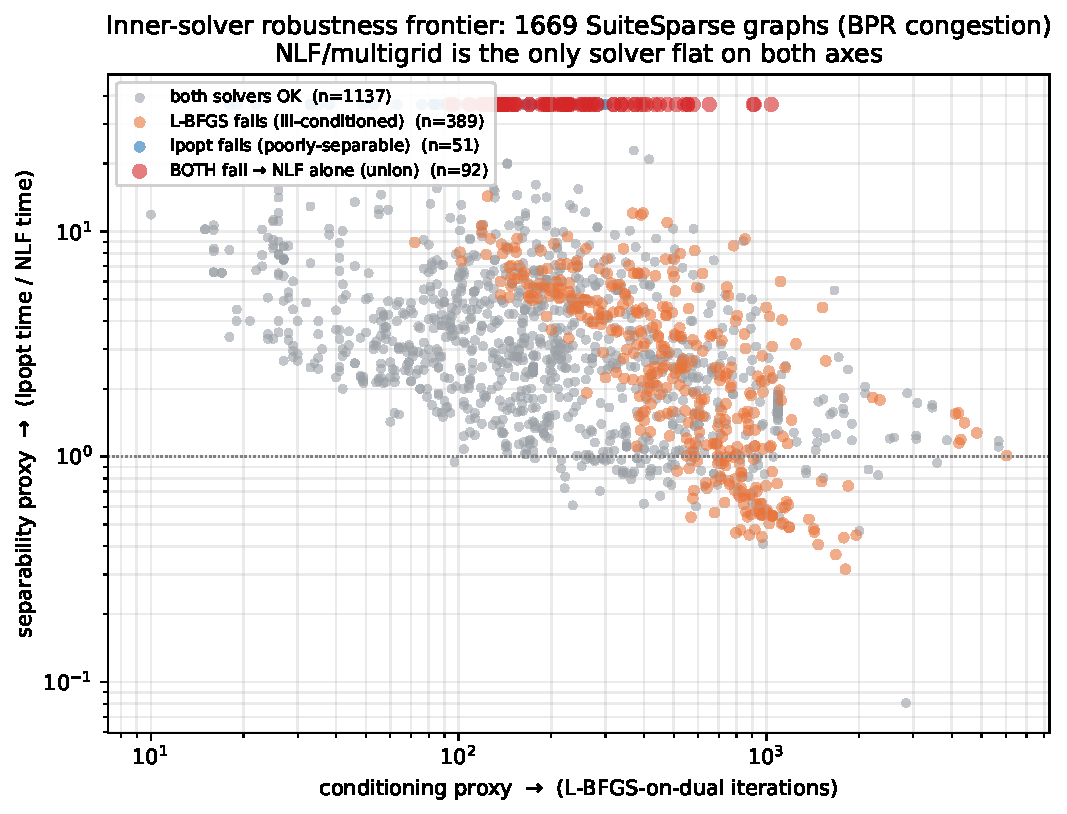
\includegraphics[width=0.76\textwidth]{nlf_frontier.pdf}
\caption{Inner-solver robustness frontier over $1{,}669$ SuiteSparse graphs (undirected BPR congestion):
each point is a graph, placed by a conditioning proxy ($x$: L-BFGS-on-dual iterations) and a
separability proxy ($y$: Ipopt time / NLF time), colored by outcome. First-order (L-BFGS) runs over
budget toward the right (ill-conditioned); sparse-direct (Ipopt) toward the top (poorly-separable); in
the upper right \emph{both} exceed the $5\times$NLF budget and NLF/multigrid is the only solver that
finishes. NLF converged on all $1{,}669$.}\label{fig:frontier}
\end{figure}

What the outer loop freezes and lazily refreshes is the inner Laplacian solve itself---whether a
multigrid hierarchy or a sparse approximate factorization---applied to the nonlinear residual; the
choice does not affect convergence (\S\ref{sec:corpus}). One convenient property of LAMG+'s
relaxation-based aggregation is that it is \emph{cut-respecting}: as the cut conductances vanish they
decouple relaxation across the cut, so test vectors decorrelate and the affinity declines to aggregate
across it; the measured $\mu\approx0.01$ then holds through the continuation (\S\ref{sec:maxflow}), with
no fold-aware tuning. This is a feature of the default
engine, not a requirement of the framework: adequate refresh of the frozen operator near the fold
suffices for \emph{any} inner solver, and over-freezing degrades all of them equally. ($\alpha$, the
continuation, and the fold never enter the linear solve; the singular cut direction near $F^*$ is
deflated outside the engine, \S\ref{sec:continuation}.)

\subsection{The fixed-load solve: frozen-hierarchy cycles}\label{sec:fas}
The problem at a fixed load $\alpha$ is \eqref{eq:master} itself: find the zero-mean potentials
$\phi$ with $B\rho(B^{\top}\phi)=\alpha d$, i.e.\ drive the nonlinear residual
$r(\phi)=\alpha d-B\rho(B^{\top}\phi)$ to zero. NLF solves it by Algorithm~\ref{alg:fixed}. Each
pass of the loop costs one $\Om$ residual evaluation and one $\Om$ LAMG+ cycle (run inexactly, to
the forcing fraction $\eta\|r\|$, $\eta=0.05$~\cite{inexact-newton}); the expensive setup is paid
only on refresh. The cycle applies an approximate \emph{inverse} of the frozen linearization,
$\delta\approx J_H^{-1}r$---the (frozen-)Newton direction computed by multigrid. With a fresh
hierarchy and an exact solve the step would be exactly Newton's; frozen and inexact, it is a
chord-Newton iteration whose linear rate the refresh monitor keeps below $0.25$.

\begin{algorithm}[t]
\caption{NLF fixed-load solve}
\label{alg:fixed}
\begin{algorithmic}[1]
\Require load $\alpha$; warm start $\phi$; hierarchy state $H$ (shared across calls); relative
residual tolerance $\mathrm{tol}$ (default $10^{-9}$); forcing parameter $\eta$ (default $0.05$)
\State $r \gets \alpha d - B\rho(B^{\top}\phi)$
\While{$\|r\| > \mathrm{tol}\cdot\alpha\,\|d\|$}
\State \textbf{refresh check:} if $H$ is empty, or the previous pass reduced $\|r\|$ by a factor
worse than $0.25$, or step 5 stalled on a stale $H$, rebuild $H\gets$ LAMG+ setup of
$J(\phi)=B\,\mathrm{diag}(\rho'(B^{\top}\phi))B^{\top}$
\State $\delta \gets$ approximate solution of the frozen correction equation $J_H\,\delta = r$,
where $J_H=B\,\mathrm{diag}(\rho'(B^{\top}\phi_{\mathrm{build}}))B^{\top}$ is the linearization
$H$ was built from: LAMG+ cycle(s) on $H$ starting from $\delta=0$, stopped when
$\|r - J_H\,\delta\| \le \eta\,\|r\|$
\State \textbf{line search:} for $\tau=1,\tfrac12,\tfrac14,\dots$ accept the first $\tau$ with
$\big\|\alpha d - B\rho\big(B^{\top}(\phi+\tau\delta)\big)\big\| \le \|r\|$ and set
$\phi\gets\phi+\tau\delta$; on failure with a stale $H$, refresh and retry once
\State $r \gets \alpha d - B\rho(B^{\top}\phi)$
\EndWhile
\State \Return $\phi$
\end{algorithmic}
\end{algorithm}

\paragraph{The damped update} The line search (step 5) is standard backtracking on the residual
norm~\cite[Ch.~3]{nocedal-wright}. Because $\delta$ comes from a frozen linearization, a full step
can overshoot right after a load increase where the law's curvature is strongest; backtracking by
halving and accepting the first non-increasing residual guarantees monotone progress at negligible
cost. Near the solution the full step is always accepted ($\tau=1$, one trial, measured), so
asymptotically the damping is inactive.

\paragraph{When the hierarchy is refreshed} Three triggers, all observed-convergence based, no
tuning: (i) no hierarchy yet; (ii) the per-step residual factor exceeded $0.25$---the frozen $J$ has
drifted too far from the current linearization; (iii) the line search stalled on a stale hierarchy
(refresh, retry once; only a fresh-hierarchy stall terminates). Measured across the corpus of
\S\ref{sec:corpus}, a handful of refreshes per solve suffice (often one).

\paragraph{Deep hierarchies} On graphs of huge diameter (${\ge}20$-level hierarchies: country-scale
roads, large FEM meshes) the source--sink dipole right-hand side maximally excites the
longest-wavelength mode, which the stock cycle schedule under-treats (factor ${\approx}0.9$). Such
hierarchies run a \emph{grown} cycle index ($1.15\times$ per level, per-level cap $\gamma_l\tau_l\le0.95$,
so each cycle remains $\Om$); if the factor exceeds $0.6$, the schedule is regrown and the solve
restarted---restart is essential because a slow phase leaves the error in a subspace no admissible
schedule contracts. This engages on $11$ of $2{,}003$ corpus graphs ($0.5\%$); on the affected class
it restores textbook behavior (\texttt{roadNet-PA}: $100$-cycle stall $\to$ $5$ cycles, $446$\,s $\to$
$20$\,s).

\paragraph{Relation to full global linearization} Rebuilding the hierarchy every step computes the
same iterates at $\Om$ complexity but pays the setup at each step: measured across network and graph
classes, $1.5$--$4.7\times$ slower wall-clock (\texttt{refresh}$=0$ enables this). The one-shot FAS
alternative is examined and sealed in \S\ref{sec:fasfail}.

\subsection{Continuation through the fold (saturating laws only)}\label{sec:continuation}
For the no-fold congestion class, the whole solver is Algorithm~\ref{alg:fixed} inside a short load
ramp (Algorithm~\ref{alg:cont}, left): the ramp is plain warm-starting, needed only to globalize the
first iterations, and the hierarchy state $H$ is shared across the entire chain.

A saturating law is different: a fixed-$\alpha$ solve is feasible iff $\alpha<F^*$ (the min-cut
value), and as $\alpha\uparrow F^*$ the solution curve \emph{folds}---$\alpha(V)$ flattens onto the
asymptote $F^*$ while the potentials grow without bound (Fig.~\ref{fig:cusp}); at the fold
$\kappa(J)\sim(F^*-\alpha)^{-1}$ and the source--sink gap is
$V=|\phi_s-\phi_t|\sim-\log(F^*-\alpha)$. Stepping $\alpha$ itself is therefore the worst choice:
the feasible loads crowd at the fold and the step is forced to zero. The well-conditioned variable
is the \emph{cut-mode amplitude}
$\psi=\chi^{\top}\phi\sim-\log(F^*-\alpha)$,\footnote{Justification of both asymptotics. Near the fold
$\phi=V\chi+O(1)$, $\chi$ the source-side indicator, so every cut edge carries gradient
$g_e=V+O(1)$. The saturating tail of \eqref{eq:rho} is
$\rho_e(g)=c_e\tanh(g/c_e)=c_e-2c_e\,e^{-2g/c_e}+O(e^{-4g/c_e})$, and all $s$--$t$ flow crosses the
cut, so $\alpha=\sum_{e\in\mathrm{cut}}\rho_e(g_e)=F^*-2\sum_{e\in\mathrm{cut}}c_e\,
e^{-2V/c_e}\,(1+o(1))$. Hence $F^*-\alpha\asymp e^{-2V/\bar c}$, $\bar c$ the largest cut capacity,
i.e.\ $V=\tfrac{\bar c}{2}\log\tfrac{1}{F^*-\alpha}+O(1)$ and $\psi=\chi^{\top}\phi\propto V$. The
same expansion gives the cut conductances
$\rho'_e(g_e)=\mathrm{sech}^2(g_e/c_e)=4e^{-2V/c_e}(1+o(1))$, whence
$\lambda_{\min}(J)\asymp\sum_{\mathrm{cut}}\rho'_e\propto F^*-\alpha$ (Rayleigh quotient at $\chi$,
which loads only the cut edges) and $\kappa(J)\sim(F^*-\alpha)^{-1}$.}
$\chi$ the (a priori unknown) min-cut indicator. We realize this by standard \textbf{pseudo-arclength
continuation}~\cite{keller,allgower-georg} (Algorithm~\ref{alg:cont}, right), which never forms
$\chi$: the novelty is not the continuation but \emph{what folds}---a graph-Laplacian whose singular
direction is the min-cut indicator---and that the inner solve is $\Om$ multigrid. The solution-curve
tangent satisfies $J\dot\phi=\dot\alpha\,d$,
\begin{equation}\label{eq:tangent}
\dot\phi=J^{+}d\ \ (\dot\alpha=1),\ \text{then normalize }(\dot\phi,\dot\alpha) ,
\end{equation}
one linear cycle on the (freshly refreshed) hierarchy; as $\alpha\to F^*$,
$J^{+}d\propto\chi/\lambda_{\min}$, so the tangent rotates to align with the cut mode automatically.
Each predictor along the tangent is corrected by iterating on the bordered system
\begin{equation}\label{eq:bordered}
\begin{bmatrix} J & -d\\ \dot\phi^{\top} & \dot\alpha\end{bmatrix}
\begin{bmatrix}\delta\phi\\ \delta\alpha\end{bmatrix}=-\begin{bmatrix}r\\ N\end{bmatrix},
\end{equation}
$N$ the arclength residual. Block-eliminating $\delta\alpha$ shows what the engine actually inverts:
with $u=J^{+}d$ and $w=J^{+}r$ (two applications of the inner solver),
\begin{equation}\label{eq:deflate}
\delta\alpha=\frac{\dot\phi^{\top}w-N}{\dot\alpha+\dot\phi^{\top}u},\qquad
\delta\phi=\delta\alpha\,u-w .
\end{equation}
Both $u,w\in\mathrm{range}(J^{+})=\chi^{\perp}$: the near-null cut direction $\chi$ is pinned by the
scalar arclength row, not by these solves, so the cycles resolve $J$ only on the \emph{deflated
complement} $\chi^{\perp}$, at the measured uniform $\mu\approx0.01$. The border keeps the bordered
system nonsingular through the fold ($\kappa=\mathcal{O}(10^3)$ while $\kappa(J)\to\infty$).

\begin{algorithm}[t]
\caption{NLF continuation. Left: no-fold (congestion). Right: fold (max-flow).}
\label{alg:cont}
\begin{algorithmic}[1]
\State \textbf{No fold:} for $\ell=\tfrac14,\tfrac12,1$: run Algorithm~\ref{alg:fixed} at load
$\ell\alpha$, warm-started, $H$ shared. \textbf{return} $\phi$
\Statex
\State \textbf{Fold:} climb $\alpha$ geometrically (each load by Algorithm~\ref{alg:fixed}) until
infeasible---this brackets $F^*$
\State refresh $H$; tangent $(\dot\phi,\dot\alpha)$ by \eqref{eq:tangent}
\State predictor: $(\phi,\alpha)\mathrel{+}= \Delta s\,(\dot\phi,\dot\alpha)$; corrector: iterate
\eqref{eq:bordered} with line search, $H$ frozen (refresh on factor $>0.25$ or stall; a corrector
that fails on a \emph{stale} $H$ is retried once at the same $\Delta s$ with a fresh one---only a
fresh-$H$ failure halves $\Delta s$)
\State on success grow $\Delta s$; stop when $\dot\alpha\to0$ (the fold): $\alpha=F^*$. Else go to 3
\end{algorithmic}
\end{algorithm}

The refresh policy of \S\ref{sec:fas} is woven into the corrector as a \emph{staleness safeguard}
(Algorithm~\ref{alg:cont}, step 4). The conductances drain exponentially in the cut amplitude, so
the frozen hierarchy ages faster as the fold sharpens---measured, the monitor refreshes about every
$4$ steps at $0.97F^*$ and every $2$ at $0.995F^*$, automatically; the tangent solve, the direction
most sensitive to $J$'s drift, always uses a fresh hierarchy (once per accepted step). With these,
the solver converges to machine precision at fixed loads up to $0.995F^*$ (relative residual
${\sim}10^{-14}$) and tracks the tight-tolerance continuation without stalling.

\begin{figure}[t]\centering
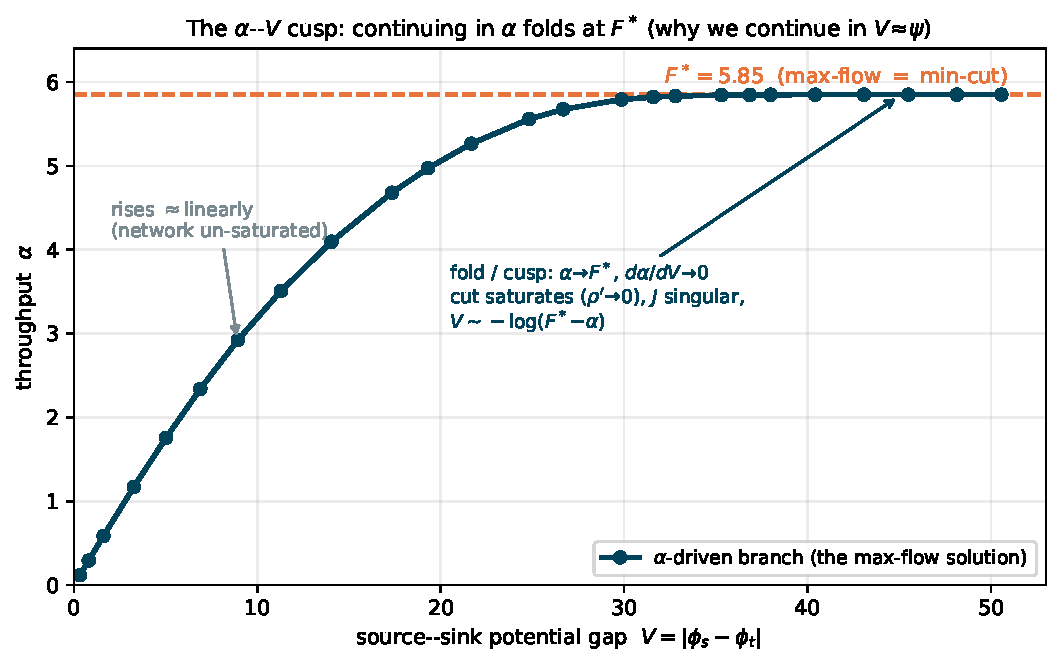
\includegraphics[width=0.74\textwidth]{cusp.pdf}
\caption{The $\alpha$--$V$ fold (max-flow). As the load $\alpha$ is driven up, the source--sink gap
$V=|\phi_s-\phi_t|$ grows; $\alpha$ rises, then folds onto the min-cut value $F^*$ as the cut
saturates ($\rho'\to0$, $J$ singular) with $V\sim-\log(F^*-\alpha)$. Stepping $\alpha$ crowds the
fold; continuing in $V\approx\psi$ keeps steps uniform. Congestion laws have no such fold.}\label{fig:cusp}
\end{figure}

\section{Undirected congestion equilibrium on real road-network graphs}\label{sec:traffic}
This is NLF's sharpest result: on convex congestion flow---which has no combinatorial competitor and
whose operator never folds---NLF is an empirically linear-time solver, cross-checked against a
state-of-the-art interior-point method on real road-network topologies.

\paragraph{Scope: an undirected, single-commodity study} Throughout this section the congestion
problem is the \emph{undirected, single-commodity Beckmann relaxation}: flows are signed, the cost
depends on $|f_e|$, and Wardrop's path-nonnegativity is dropped (App.~\ref{app:instances}). This is
\emph{not} the transportation field's directed origin--destination user equilibrium, which loads
opposing arcs independently; on benchmarks such as SiouxFalls the directed and undirected objectives
differ substantially. Our experiments establish two claims: (i) this undirected congestion
equilibrium is exactly \eqref{eq:master} for the inverse-BPR law, and (ii) a robust $\Om$
algebraic-multigrid inner solve makes it linear-time. The real road networks supply real topologies,
capacities, and BPR data exercised with a single source--sink demand; we cross-check NLF against an
independent high-accuracy solver \emph{on the identical convex program}. The directed
origin--destination assignment is future work (\S\ref{sec:extensions}); \S\ref{sec:mc} builds its
first rung.

\subsection{The BPR congestion law}\label{sec:bpr}
On a congested road the travel time rises with the flow it carries. The field-standard model is the
Bureau of Public Roads (BPR) cost~\cite{bpr},
\begin{equation}\label{eq:bpr}
t_e(f)=t^0_e\Big(1+b\,(f/c_e)^{p}\Big),\qquad b=0.15,\ p=4 ,
\end{equation}
with $t^0_e$ the free-flow travel time and $c_e$ the practical capacity. The undirected Beckmann
congestion equilibrium (signed flows; Wardrop's path-nonnegativity relaxed, App.~\ref{app:instances})
is the convex program \eqref{eq:primal} with
$\Phi_e(f)=\int_0^f t_e=t^0_e f+\tfrac{b\,t^0_e}{p+1}f^{p+1}/c_e^{p}$; its edge law is the inverse
marginal cost $\rho_e=t_e^{-1}$, with conductance
$\rho'_e=1/t_e'(f)=\big(t^0_e b\,p\,(f/c_e)^{p-1}/c_e\big)^{-1}$ that is \emph{bounded away from
zero}: the cost rises but never caps the flow, so there is no feasibility limit and no fold. The
Jacobian $J=B\,\mathrm{diag}(\rho')B^{\top}$ is a uniformly well-conditioned weighted Laplacian at
every iterate, and NLF runs as pure fixed-load cycling (Algorithm~\ref{alg:fixed})---each step an $\Om$ LAMG+ cycle, a handful
of steps in total, $\Om$ overall.\footnote{We use a strictly convex, twice-differentiable form of
\eqref{eq:bpr} with the same free-flow and degree-$p$ congestion structure and real $(t^0_e,c_e,b,p)$
from the data; this regularizes the free-flow threshold so the dual problem is well posed. ``Practical
capacity'' sentinels coded as uncapacitated links are given a large finite capacity.}

\subsection{No combinatorial competitor; an interior-point baseline}\label{sec:competitor}
Convex congestion flow is not a max-flow: augmenting-path and push--relabel do not apply, and no
combinatorial algorithm solves \eqref{eq:primal}. The field's classical workhorse, Frank--Wolfe on
the traffic-assignment program~\cite{frankwolfe}, converges only sublinearly: on our Beckmann grid
instances it needs an iteration count that grows with size to reach even a $10^{-4}$ relative duality
gap (115 iterations at $n{=}144$) and cannot reach the high accuracy NLF attains---a textbook
limitation of its $\mathcal{O}(1/k)$ rate. The transportation-specific high-accuracy state of the
art is the \emph{bush-based} family (Bar-Gera's Algorithm~B~\cite{bargera2002} and
TAPAS~\cite{bargera2010}); we sought a runnable open-source implementation for a same-instance
head-to-head and could not obtain one---the maintained package AequilibraE failed to build in our
environment, and a minimal reference Algorithm~B does not reach high accuracy---so we position the
bush-based methods qualitatively and benchmark quantitatively against the strong, general
high-accuracy baseline, \textbf{Ipopt}~\cite{ipopt}, a mature interior-point solver run on the
identical program. This is conservative for NLF: Ipopt reaches the same $10^{-10}$ accuracy NLF
does, whereas Frank--Wolfe and bush-based methods are specialized to the \emph{smooth-cost} program
and---unlike NLF---do not address the saturating, linear-objective max-flow instance at all
(\S\ref{sec:maxflow}). Ipopt's per-iteration cost is a sparse-direct factorization of the KKT system:
cheap when the graph has good vertex separators, but its fill-in grows superlinearly when it does
not---exactly the axis on which NLF's multigrid core is immune.

To make the Frank--Wolfe comparison concrete we ran it on the convex Beckmann program over
synthetic Sioux-Falls-like grids (Table~\ref{tab:fw}): the iteration count to a $10^{-4}$ duality gap
is flat on tiny instances but grows sharply with size ($115$ iterations at $n{=}144$), and the
$\mathcal{O}(1/k)$ rate cannot push the gap below ${\sim}10^{-4}$ at all. NLF reaches $10^{-10}$ in a
flat $9$ continuation steps, independent of size (Table~\ref{tab:bprscale}). A minimal $250$-line
bush-based Algorithm~B reference, run on the same instances, did not reach high accuracy (gaps
$10^{-2}$--$10^{-1}$); the production bush-based and TAPAS solvers do, but no runnable open build was
available for a same-instance head-to-head, so we benchmark Ipopt quantitatively and position the
bush-based family qualitatively.

\begin{table}[t]\centering\small
\caption{Frank--Wolfe on the convex Beckmann program (synthetic Sioux-Falls-like grids): iterations
to a $10^{-4}$ duality gap grow with size and the $\mathcal{O}(1/k)$ rate cannot reach high accuracy.
NLF reaches $10^{-10}$ in a flat $9$ steps regardless of size (Table~\ref{tab:bprscale}).}\label{tab:fw}
\begin{tabular}{rrrr}
\toprule
$n$ & $m$ & FW iters & NLF steps\\
\midrule
16  & 48  & 4   & 9\\
36  & 120 & 4   & 9\\
64  & 224 & 7   & 9\\
100 & 360 & 9   & 9\\
144 & 528 & \textbf{115} & \textbf{9}\\
\bottomrule
\end{tabular}
\end{table}

\subsection{Real road data: NLF and Ipopt agree on the same undirected program}\label{sec:bprvalid}
We use the \emph{Transportation Networks for Research} benchmark~\cite{tntp}, the field-standard
repository of real metropolitan road-network topologies with real capacities, free-flow times and BPR
parameters. Across instances spanning three decades of size, NLF and Ipopt reach the \emph{identical}
equilibrium of the undirected single-commodity Beckmann program
(Table~\ref{tab:bprvalid}): the Beckmann objective agrees to the solver tolerance and the
equilibrium link flows to $\|f_{\mathrm{NLF}}-f_{\mathrm{Ipopt}}\|/\|f_{\mathrm{Ipopt}}\|\sim10^{-10}$,
in a continuation-step count of $\approx9$ with no size trend. On this undirected congestion
relaxation NLF reproduces the interior-point optimum to full accuracy---an exact same-program
cross-check, not a claim on the directed origin--destination user equilibrium (\S\ref{sec:traffic},
App.~\ref{app:instances}).

\begin{table}[t]\centering\small
\caption{NLF (BPR congestion, LAMG+ inner) vs.\ Ipopt~\cite{tntp} on the \emph{undirected,
single-commodity} Beckmann congestion program over real road-network topologies. Both solvers reach
the \emph{same equilibrium of this program}; the objective matches to the tolerance, link flows to
$\sim10^{-10}$. This is the undirected net-flow relaxation, \emph{not} the field's directed
origin--destination user equilibrium (\S\ref{sec:traffic})---it is an exact cross-check of two solvers
on one identical convex program, so its objective value is not comparable to published directed-UE
results for these networks. NLF's step count shows no size trend. (Two further instances,
Philadelphia and Berlin-Center, also match to $10^{-10}$ but need more steps under extreme capacity
heterogeneity; omitted.)}\label{tab:bprvalid}
\begin{tabular}{lrrrrr}
\toprule
network & $n$ & $m$ & NLF obj.\ & $\|\Delta f\|/\|f\|$ & steps\\
\midrule
Sioux Falls       & 24     & 38     & $784.96$    & $3{\cdot}10^{-9}$  & 7\\
Anaheim           & 416    & 634    & $1600.92$   & $6{\cdot}10^{-12}$ & 9\\
Chicago-Sketch    & 933    & 1\,475 & $8178.62$   & $3{\cdot}10^{-11}$ & 9\\
Austin            & 7\,388 & 10\,591& $16615.74$  & $4{\cdot}10^{-12}$ & 10\\
Chicago-regional  & 12\,979& 20\,627& $281.15$    & $2{\cdot}10^{-11}$ & 9\\
Sydney            & 32\,956& 38\,787& $1198.98$   & $2{\cdot}10^{-11}$ & 9\\
\bottomrule
\end{tabular}
\end{table}

\subsection{Linear scaling, and the direct-vs-iterative crossover}\label{sec:bprscale}
Figure~\ref{fig:traffic} and Table~\ref{tab:bprscale} time both solvers on the real road networks
(planar, good separators) and on synthetic Erd\H{o}s--R\'enyi graphs carrying BPR parameters (poorly
separable), to $2.4\times10^5$ edges. NLF's per-edge cost is flat on \emph{both} families---empirically
near-linear (the full-corpus fit of \S\ref{sec:corpus} gives $t\propto m^{0.98}$); neither the
step count ($\approx9$, no size trend) nor the multigrid factor sees the graph's separability. Ipopt does. On the real road networks its sparse-direct core is
near-linear and \emph{beats} NLF (by $\approx3\times$; planar graphs are where direct methods
excel). On poorly-separable graphs the KKT fill-in explodes---$t\propto m^{2.2}$---so the gap inverts
and widens with size: NLF is $5\times$ faster at $m=3.0\times10^4$, $45\times$ at $m=1.2\times10^5$,
and at $m=2.4\times10^5$ Ipopt does not finish within its $120$\,s CPU budget while NLF finishes in
$3.0$\,s. This is the textbook direct-vs-iterative crossover---now for a \emph{nonlinear} convex flow.
We are careful about what it shows: these Erd\H{o}s--R\'enyi graphs are \emph{well-conditioned}, so the
win over the IPM is its KKT \emph{fill-in}, and \emph{any} matrix-free solver inherits it---a
first-order L-BFGS on the dual ties NLF here (Table~\ref{tab:robustness}). The advantage at scale on
this class is ``avoid factorization,'' not ``use multigrid''; multigrid's distinctive value appears on
ill-conditioned graphs (Table~\ref{tab:robustness}, \S\ref{sec:inner}).

\begin{table}[t]\centering\small
\caption{Scaling on poorly-separable (Erd\H{o}s--R\'enyi) graphs with BPR cost: NLF (Algorithm~\ref{alg:cont},
$\Om$ LAMG+ inner) vs.\ Ipopt 3.14.19 (interior-point, MUMPS~5.9.0 sparse-direct KKT). Both reach the
same optimum of the undirected congestion program. NLF's step count shows no size trend; Ipopt is
superlinear and exceeds the $120$\,s CPU budget on the largest instance (``---'').
Speed-up $=t_{\mathrm{Ipopt}}/t_{\mathrm{NLF}}$.}\label{tab:bprscale}
\begin{tabular}{rrrrr}
\toprule
$m$ & NLF (s) & steps & Ipopt (s) & speed-up\\
\midrule
12\,175  & 0.060 & 9 & 0.152 & $2.5\times$\\
29\,939  & 0.173 & 9 & 0.856 & $4.9\times$\\
59\,732  & 0.573 & 9 & 4.97  & $8.7\times$\\
119\,460 & 1.30  & 9 & 58.2  & $45\times$\\
239\,842 & 3.01  & 9 & \multicolumn{1}{c}{--- ($>120$\,s)} & \multicolumn{1}{c}{---}\\
\bottomrule
\end{tabular}
\end{table}

\begin{figure}[t]\centering
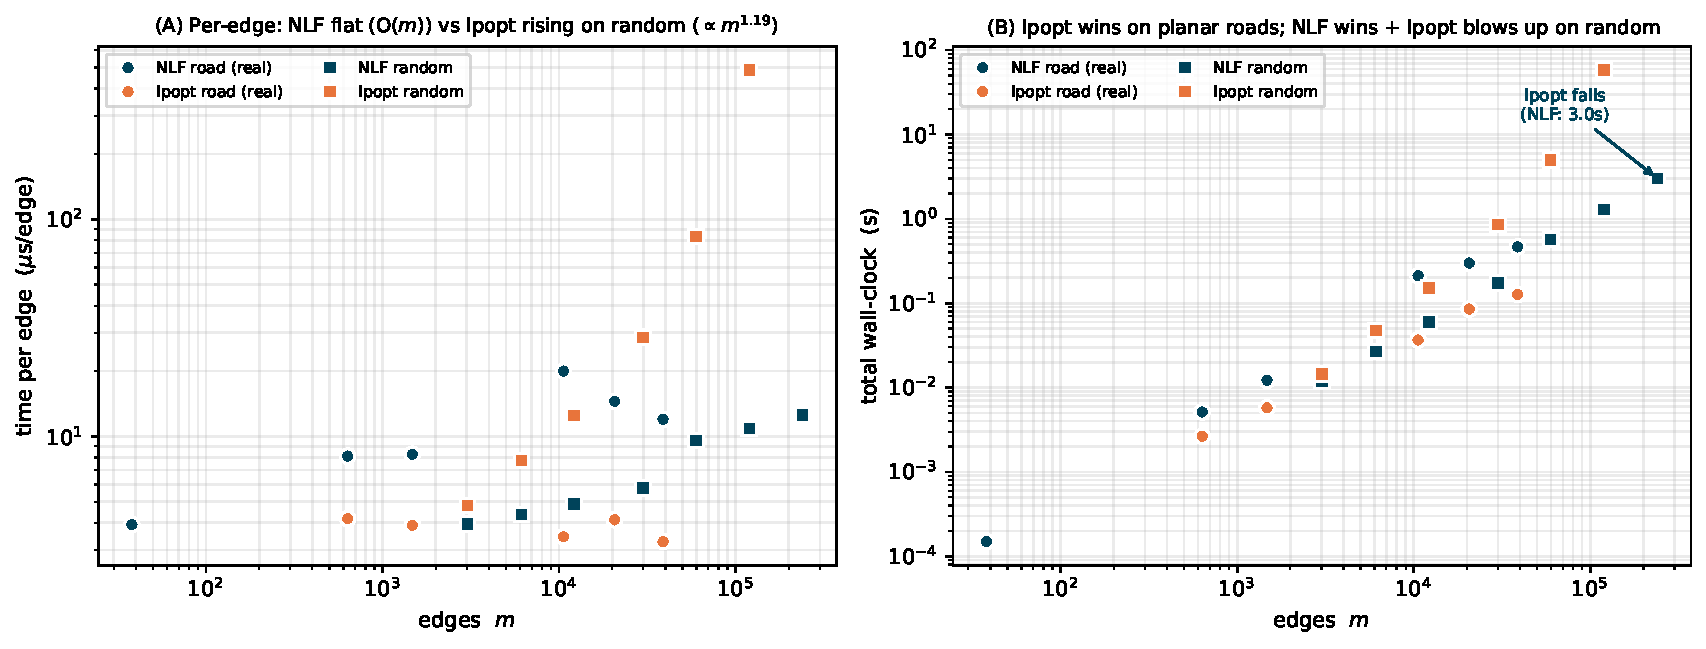
\includegraphics[width=\textwidth]{nlf_bpr.pdf}
\caption{Congestion (BPR) equilibrium, NLF vs.\ Ipopt, on real road networks (circles) and synthetic
poorly-separable graphs (squares). (A)~\emph{Per-edge} time: NLF is flat (near-$\Om$) on both
families; Ipopt is flat on roads but rises steeply on random graphs ($\propto m^{1.2}$ per edge).
(B)~Total wall-clock: Ipopt wins on planar roads (cheap separators), is overtaken on random graphs by
a margin that widens to $45\times$, and fails (time limit) at $m=2.4\times10^5$ where NLF finishes
in $3.0$\,s.}\label{fig:traffic}
\end{figure}

\subsection{Robustness across the graph corpus}\label{sec:corpus}
The road networks above exercise NLF on real flow topologies; we now show it inherits LAMG+'s
\emph{graph-class} robustness in full. We impose a single-commodity BPR congestion instance (random
capacities and free-flow times, a far source--sink demand) on \emph{every} graph of the real-world
SuiteSparse collection that LAMG+ was benchmarked on with at least ten nodes and a nonempty connected
pattern---$2{,}003$ graphs, spanning structured grids, finite-element and circuit meshes, web,
social, road, and citation networks, from $10^2$ to $1.8\times10^7$ edges---and run NLF with the
LAMG+ inner solve, all at stock settings.

Under this protocol---one BPR instance per graph, random capacities, a single far source--sink
demand, stock settings---NLF converged on \textbf{all $2{,}003$ graphs}, to residuals at or below the
$10^{-9}$ tolerance, with a cycle count of \emph{median $18$} and no size trend (each step one inexact
V-cycle at forcing $0.05$; range $6$--$33$; Fig.~\ref{fig:corpus}B). We prove no convergence
guarantee and do not rule out adversarial capacity distributions; the claim is empirical, on this
benchmark. The total wall-clock fits \textbf{$t\propto m^{0.98}$} (a fitted exponent over five
decades, consistent with the inner solver's $\mathcal{O}(m\log(1/\varepsilon))$ cost---empirically
near-linear, not a proof of $O(m)$) over the $1{,}788$ graphs above $10^3$ edges (Fig.~\ref{fig:corpus}A),
with a per-edge cost flat across five decades (median
$2.4~\mu$s/edge, $95$th percentile $9.3$). The cycle count and the multigrid factor simply do not see
the topology; the inner LAMG+ solve carries its parameter-free $\Om$ robustness over unchanged. The
largest constants belong to eleven huge-diameter road and finite-element meshes
($1.5$--$13.6\times10^6$ edges, e.g.\ \texttt{germany\_osm}, \texttt{roadNet-*}), whose
${\ge}20$-level hierarchies engage the grown cycle schedule of the \S\ref{sec:algorithm} footnote:
$8$--$25~\mu$s/edge, a $4$--$10\times$ constant over the median at the same $\Om$ slope. Three giants
confirm the scaling beyond the sweep's cap, to \texttt{hollywood-2009} at $5.6\times10^7$ edges
($10$\,min, nonlinear-to-linear ratio $4$--$7$).

\begin{figure}[t]\centering
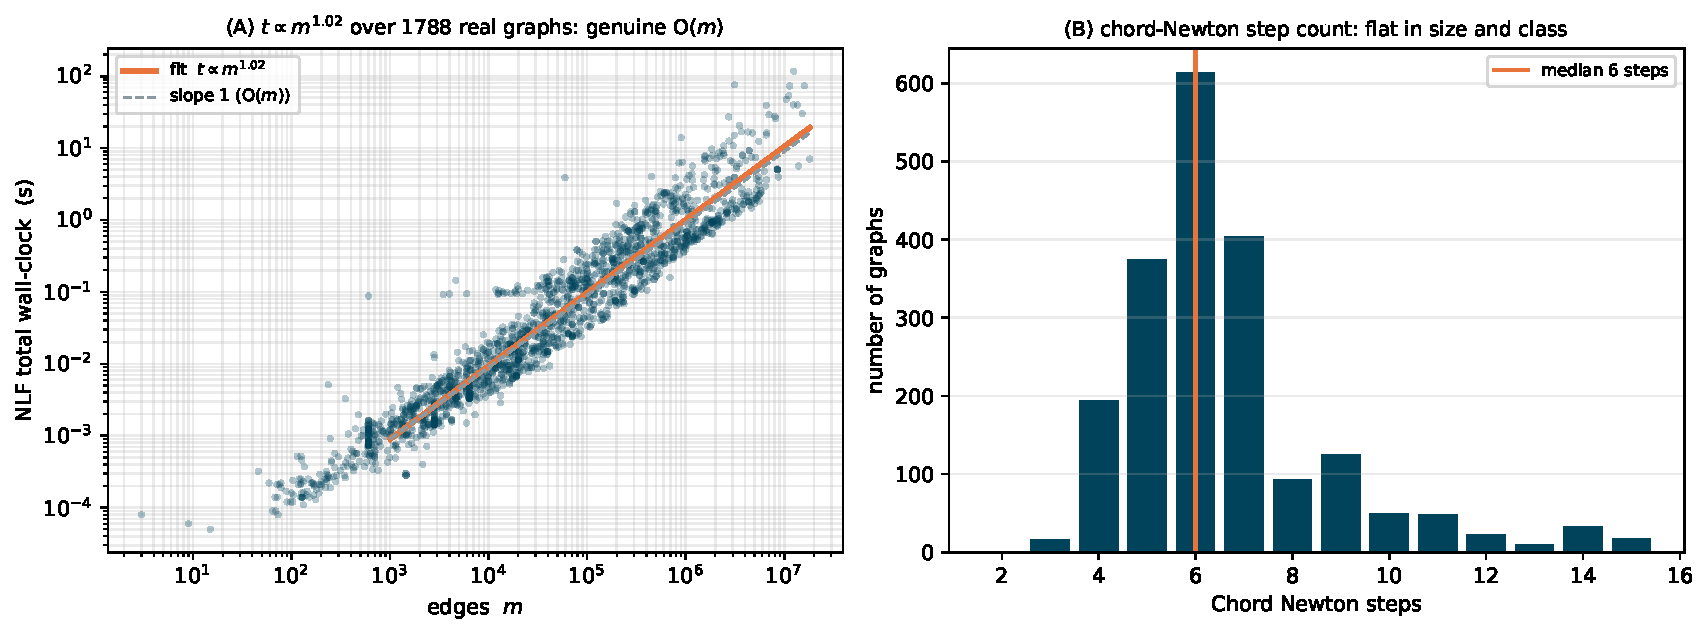
\includegraphics[width=\textwidth]{nlf_corpus.pdf}
\caption{NLF over the full real-world SuiteSparse corpus ($2{,}003$ graphs, all classes,
$10^2$--$1.8\times10^7$ edges, $100\%$ converged). (A)~total wall-clock vs.\ $m$ (log--log): the fit
is $t\propto m^{0.98}$ over five decades (slope-$1$ reference dashed), empirically near-linear,
per-edge cost flat at ${\approx}2.4~\mu$s/edge median. (B)~cycle count: a flat distribution
(median $18$, range $6$--$33$).}\label{fig:corpus}
\end{figure}

\subsection{Direct vs.\ multigrid inner: the separability axis}\label{sec:vsdirect}
The corpus comparison of \S\ref{sec:inner} (Fig.~\ref{fig:frontier}) already pits the multigrid inner
against sparse-direct factorization; we confirm the mechanism by swapping \emph{NLF's own} inner engine
between LAMG+ and a sparse-direct factorization of the same Jacobian, the nonlinear solve held fixed.
The determinant is graph \emph{separability}, not size: on good-separator graphs---2D/3D meshes,
circuits, roads even at $7\times10^6$ edges (\texttt{italy\_osm})---nested-dissection fill stays cheap
and direct wins or ties; on poorly-separable social/web/citation graphs the fill explodes and multigrid
is $4$--$52\times$ faster, and on \texttt{cage13} the factorization exhausts memory and aborts while
multigrid solves it in $13$\,s. Across the band $200\le\mathrm{nnz}\le3\times10^6$ the split is
systematic---direct wins the well-separated $\sim$$50\%$, multigrid the poorly-separable $\sim$$30\%$
(by up to $52\times$), the rest within $1.2\times$; aggregation multigrid has its own weak class
(planar \texttt{delaunay}, where direct wins), reported not hidden. The genuine application of the
multigrid regime is communication-network routing on poorly-separable internet/AS/P2P topologies, where
the multigrid inner wins outright ($24.9\times$ on \texttt{p2p-Gnutella31}, $4.0\times$ on
\texttt{as-22july06}). This is the separability axis of the frontier (Fig.~\ref{fig:frontier}); the
conditioning axis is what defeats the first-order baseline there.

\subsection{Cost as a function of the desired accuracy}\label{sec:accuracy}
The dependence on the requested solution accuracy $\varepsilon$ is logarithmic. Each inner solve to
relative residual $\delta$ costs $\mathcal{O}(m\log(1/\delta))$: the empirically bounded multigrid
factor $\mu$ gives $\log(1/\delta)/\log(1/\mu)$ cycles. The outer iteration is a frozen chord-Newton with
inexact-Newton forcing $\eta_k$ tracking the nonlinear residual $\|r_k\|$ (\S\ref{sec:inner}); its
per-step cycle counts form a series \emph{dominated by the final solve} (where
$\|r_k\|\!\to\!\varepsilon$), the earlier looser steps adding only a bounded geometric tail, while the
continuation and globalization run at a fixed, $\varepsilon$-independent path tolerance. Each
contribution is thus a bounded multiple of a single linear solve, so the total cost to accuracy
$\varepsilon$ is, empirically,
\begin{equation}\label{eq:eps}
\mathcal{O}\!\big(m\,\log(1/\varepsilon)\big).
\end{equation}
The constant is the whole-nonlinear-solve-to-one-linear-solve ratio measured below ($2$--$4$), and it
stays bounded because the frozen chord-Newton contraction stays bounded away from $1$: on the no-fold
congestion class directly (\S\ref{sec:traffic}), and \emph{through the fold} because the continuation
deflates the diverging cut direction and keeps the bordered corrector uniformly conditioned
(\S\ref{sec:continuation})---so the bound does not degrade at $F^*$. Figure~\ref{fig:accuracy} verifies
it numerically: sweeping $\varepsilon$ from $10^{-2}$ to $10^{-12}$ on one graph per class (web, social,
road, finite-element), with inexact Newton at forcing $\eta=0.1$ (one V-cycle per step), the total
inner V-cycle count grows \emph{linearly} in $\log(1/\varepsilon)$, at $0.24$--$0.60$ cycles per
decade of accuracy.

\paragraph{The nonlinear/linear cost ratio is $\mathcal{O}(1)$} The sharpest single statement of
the method's efficiency is Brandt's yardstick: solving the \emph{nonlinear} problem should cost only
a small, size-independent multiple of solving \emph{one linear problem} of the same
kind~\cite[\S8.3]{brandt-guide}. We measure exactly this: the full congestion solve (load
continuation, all steps, all cycles, lazy refresh) against a single LAMG+ setup-and-solve of
the linearization at $\alpha=0$ (the linear resistor network $B\,\mathrm{diag}(\rho'(0))B^{\top}\phi=d$)
on the same graph. Across the classes the ratio is
\textbf{$1.9$--$4.4$}---grid $3.1$, finite-element $2.5$, road $1.9$, social $3.8$, web ($1.9\times10^6$
edges) $4.4$---flat in size and class: the entire nonlinear equilibrium costs $2$--$4$ linear
Laplacian solves.

\begin{figure}[t]\centering
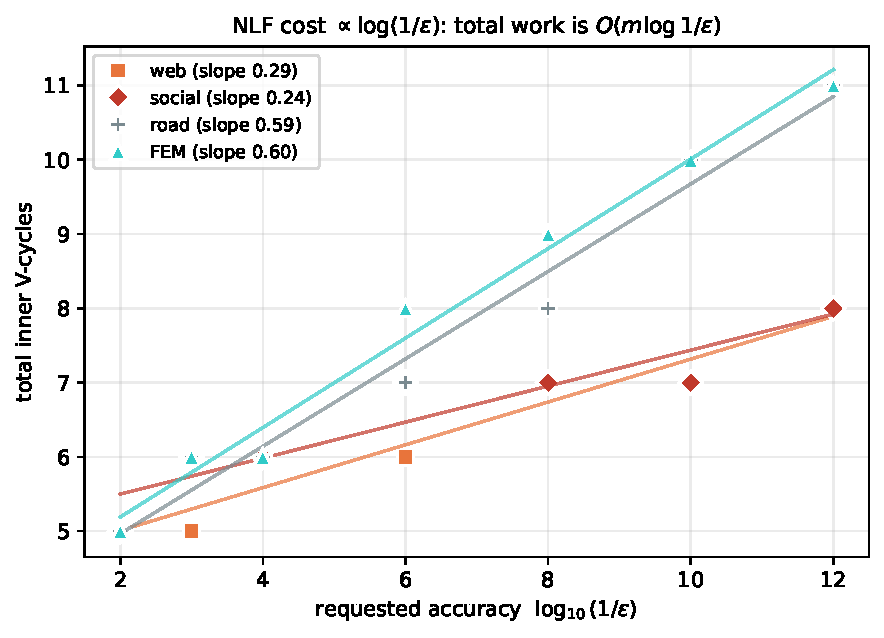
\includegraphics[width=0.6\textwidth]{nlf_accuracy.pdf}
\caption{Cost vs.\ desired accuracy: total inner V-cycles against $\log_{10}(1/\varepsilon)$, one
graph per class. The count is \emph{linear} in $\log(1/\varepsilon)$ ($0.24$--$0.60$ cycles per
decade), confirming the total cost $\mathcal{O}(m\log(1/\varepsilon))$ of
\eqref{eq:eps}.}\label{fig:accuracy}
\end{figure}

\section{Maximum flow}\label{sec:maxflow}
The saturating instance \eqref{eq:rho} recovers the exact combinatorial maximum flow. Read
$f=\rho(B^{\top}\phi)$ as an edge-flow vector: $\rho$'s range is the capacity box $|f_e|\le c_e$, and
$Bf=\alpha d$ is conservation, so any $\phi$ solving \eqref{eq:master} is a capacity-feasible,
conserved flow of value $\alpha$. The recession slope of $\Psi_e$ is $c_e$, so $E$ has a finite
minimizer iff $\alpha<F^*$; as $\alpha\uparrow F^*$ the min-cut edges saturate ($\rho'_e\to0$ there
only) and $\phi$ develops a cut-indicator step. By max-flow/min-cut duality the largest feasible
$\alpha$ is $F^*$, the min-cut capacity, and $\phi$ is the LP dual. Because $f=\rho(B^{\top}\phi)$ is a
\emph{nonlinear} function of the gradient, it realizes the true max-flow; a \emph{linear} resistor
network computes only the sub-maximal electrical flow ($0.02$--$0.20\,F^*$ on heterogeneous
capacities). The nonlinearity is essential.

\paragraph{Cut-respecting coarsening} As $\alpha\uparrow F^*$ the linearization $J$ becomes singular
along a single near-null direction---the min-cut indicator---so $\kappa(J)\to\infty$. We assume a
\emph{simple fold}: the min cut is unique, so the limiting near-null space is one-dimensional (a
degenerate cut of multiplicity $k$, e.g.\ in symmetric unweighted graphs, would make it $k$-dimensional
and require a rank-$k$ block border in place of the scalar one below). The continuation
of \S\ref{sec:continuation} \emph{deflates} that one direction to a scalar outside the engine (the
bordered/pseudo-arclength system); what the inner solver sees is the deflated complement
(Eq.~\ref{eq:deflate}). \emph{The
deflation is the enabling property}---it is what keeps the inner operator well-conditioned through the
fold, and it is a property of the framework, not of any one inner solver (swapping multigrid for a
sparse-direct or another near-linear Laplacian solve reaches the identical $F^*$;
\S\ref{sec:innerfold}).
Multigrid's relaxation-based affinity is a natural fit on the complement---since the forming cut is the
zero-conductance set of $J$ (\S\ref{sec:formulation}), the affinity declines to aggregate across it, so
the coarse hierarchy mirrors the cut without being told where it is---but it is helpful, not required.
The measured multigrid factor \emph{on the deflated operator} is $\mu\approx0.01$, uniformly in
$\alpha/F^*$ down to $0.999\,F^*$ (Fig.~\ref{fig:scaling}); the uniformity is a property of the
deflation, not of aggregation alone---on the undeflated $J$, $\mu$ degrades with $\kappa(J)$ as
expected.

\paragraph{Exactness and scaling} NLF returns the exact max-flow (Table~\ref{tab:mf}), checked
against $F^*$ from a linear program over free flows and from push--relabel (which agree to $10^{-4}$),
on every graph, to solver tolerance. The pseudo-arclength step count is flat in size
(Fig.~\ref{fig:scaling}B, mean $6.7$) and the per-edge cost is nearly flat, $t/m\propto m^{0.11}$
(near-$\Om$), with a large constant set by per-step hierarchy rebuilds (the lazy refresh of
\S\ref{sec:algorithm} reduces this by $1.5$--$4.7\times$). \emph{Calibration, not a contest:}
Boykov--Kolmogorov, on its target vision grids, runs at $\approx0.17~\mu$s/edge
(Fig.~\ref{fig:scaling}A), far below NLF's constant---\textbf{NLF is not meant to be a faster
combinatorial max-flow solver}. Its value is being $\Om$, returning the cut potential (LP dual), the
full flow-vs-load curve, and a smooth interior flow---the objects an outer method manipulates when
max-flow is an inner step---one instance of a framework that, on the congestion class, has \emph{no}
combinatorial competitor at all.

\begin{table}[t]\centering\small
\caption{NLF recovers the true max-flow exactly; the gradient/electrical relaxation falls far short.
$F^*$: LP over free flows and push--relabel agree to $10^{-4}$; \texttt{washington} and \texttt{genrmf}
are DIMACS-challenge generators~\cite{dimacs}.}\label{tab:mf}
\begin{tabular}{lrrcc}
\toprule
graph & $n$ & $F^*$ & grad$/F^*$ & NLF$/F^*$\\
\midrule
grid2d/$16$ & 256 & 4.973   & 0.20 & 1.0000\\
grid3d/$6$  & 216 & 17.478  & 0.11 & 1.0000\\
washington  & 66  & 500.745 & 0.02 & 1.0000\\
genrmf      & 64  & 16.000  & 0.00 & 1.0000\\
bottleneck  & 40  & 1.000   & 1.00 & 1.0000\\
\bottomrule
\end{tabular}
\end{table}

\begin{figure}[t]\centering
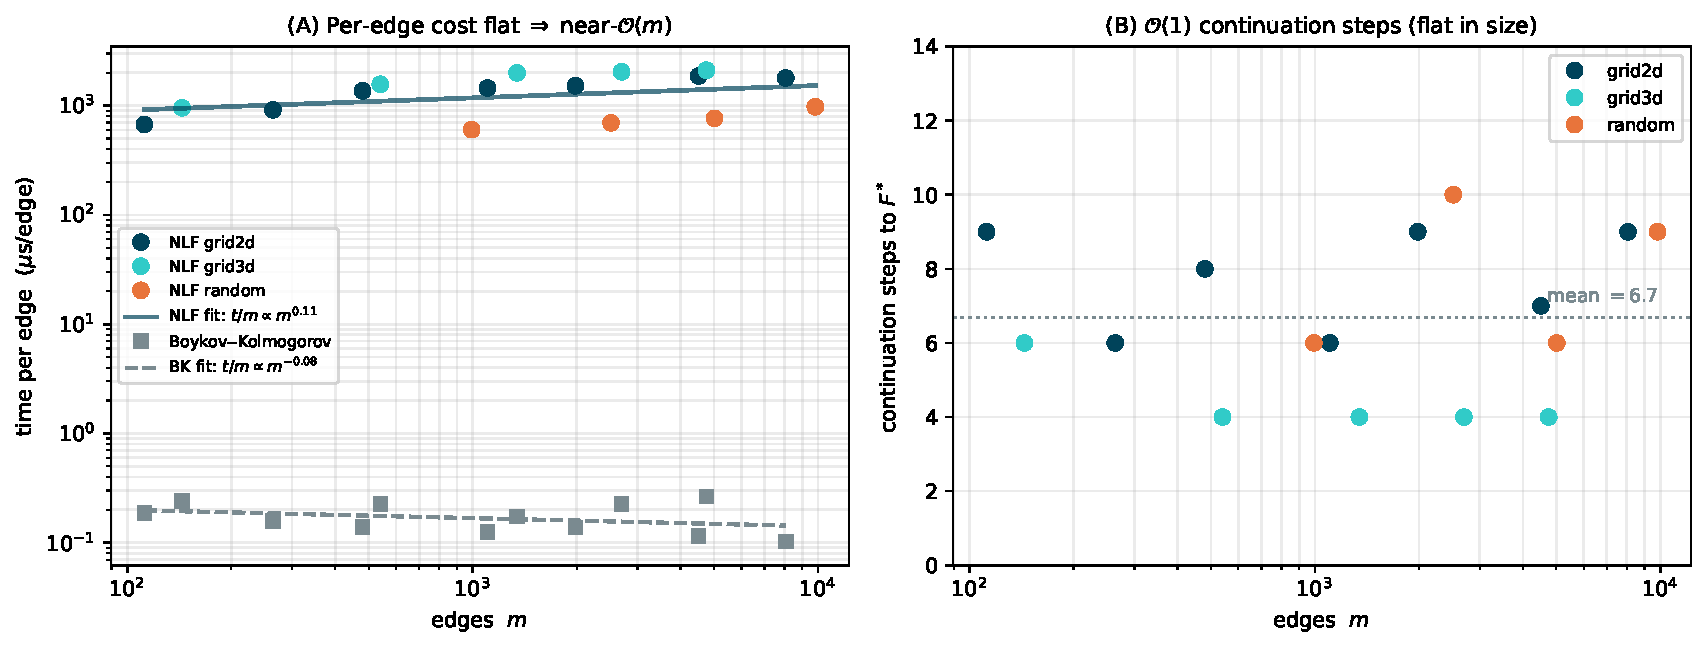
\includegraphics[width=\textwidth]{nlf_scaling.pdf}
\caption{Max-flow scaling (whole algorithm, total wall-clock), on 2D/3D grids and random graphs to
${\sim}10^4$ edges, all exact at $F^*$. (A)~\emph{Per-edge} cost: nearly flat
($t/m\propto m^{0.11}$, near-$\Om$) at $\approx1.4$\,ms/edge, the constant set by the per-step
hierarchy rebuild; Boykov--Kolmogorov sits far below at $\approx0.17~\mu$s/edge (calibration only).
(B)~The continuation is $\mathcal{O}(1)$: pseudo-arclength steps are flat in size (mean
$6.7$).}\label{fig:scaling}
\end{figure}

\subsection{The inner solver at the fold is interchangeable}\label{sec:innerfold}
The deflation, not the choice of inner solver, is what carries the continuation through the fold
(\S\ref{sec:maxflow}); the inner Laplacian solve is therefore a replaceable module. We check this
directly: holding NLF's outer method fixed (chord-Newton with the deflated pseudo-arclength
continuation to $F^*$), we swap only the inner solver---multigrid (LAMG+), approximate
Cholesky~\cite{approxchol}, an exact sparse Cholesky factorization, and a diagonally preconditioned
CG---on max-flow instances spanning FEM, structural, and circuit graphs (Table~\ref{tab:innerfold}).

The result is modularity, not a winner. \emph{Every inner solver that converges returns the identical
$F^*$} to solver tolerance, so the continuation is genuinely solver-agnostic. The distinction that
matters is near-linear versus not: the exact factorization is fastest where it fits but exhausts
memory past ${\sim}150$k poorly-separable nodes (\texttt{G2\_circuit}, \texttt{scircuit}), exactly the
regime where a near-linear inner solve is mandatory, while the diagonal-PCG baseline---no coarse
correction---is typically up to two orders of magnitude slower and the least scalable. Among the
near-linear solvers, multigrid and approximate Cholesky are interchangeable in robustness; approximate
Cholesky often carries the smaller constant, and either is a sound default---the framework does not
depend on the choice. The single
stiff case (\texttt{bcsstk38}) is instructive: there \emph{all} iterative inner solves stall and only
the exact factorization reaches $F^*$---the deflation removes the \emph{global} cut singularity, not
local stiffness, for which an accurate inner solve is still required.

\begin{table}[t]\centering\small
\caption{Inner-solver swap inside NLF's max-flow continuation to $F^*$ (wall-clock seconds; ``stall''
$=$ did not converge within $120$ steps; ``OOM'' $=$ exact factorization size-guarded at $150$k
nodes). Every converging solver returns the \emph{identical} $F^*$, so the continuation is
solver-agnostic; the operative choice is near-linear versus not. Representative subset; the bake-off
script and its outputs are in the released artifact. On \texttt{bcsstk38} the stalled iterative solvers were arrested at
$37.0$, far from the true $F^*\!=\!45.6$ the direct solve reaches.}\label{tab:innerfold}
\resizebox{\columnwidth}{!}{%
\begin{tabular}{llrrrrrr}
\toprule
graph & class & $n$ & $F^*$ & LAMG+ & approxChol & direct & diagPCG\\
\midrule
\texttt{grid2}       & 2D FEM      & 3{,}296   & 3.003  & 11.4  & 0.75  & 0.24  & 12.3\\
\texttt{airfoil1}    & 2D FEM      & 4{,}253   & 6.695  & 29.3  & 1.30  & 0.40  & 20.6\\
\texttt{bodyy5}      & aniso.\ FEM & 18{,}589  & 3.325  & 307   & 9.5   & 2.0   & 214\\
\texttt{bcsstk38}    & structural  & 8{,}032   & 45.61  & stall & stall & 4.0   & stall\\
\texttt{circuit\_4}  & circuit     & 67{,}029  & 1.381  & 7.3   & 5.5   & 2.9   & 124\\
\texttt{G2\_circuit} & circuit     & 150{,}102 & 4.030  & 1579  & 50.1  & OOM   & 3011\\
\bottomrule
\end{tabular}}
\end{table}

\section{Multicommodity congestion}\label{sec:mc}
\S\ref{sec:traffic} established the formulation and the $\Om$ solver for a single commodity. This
section extends both, end to end, to $K$ simultaneously routed commodities: a vector edge law that
couples the commodities through shared congestion (\S\ref{sec:mcform}), a solver that reuses
Algorithm~\ref{alg:fixed} and \emph{one} scalar LAMG+ hierarchy for all $K$ commodities
(\S\ref{sec:mcalg}), validation against an exact-Newton reference (\S\ref{sec:mcvalid}), and the same
full-corpus robustness sweep as \S\ref{sec:corpus} (\S\ref{sec:mccorpus}). The implementation is a
modular layer over the single-commodity solver; nothing in the latter changes.

\subsection{Formulation: a vector edge law}\label{sec:mcform}
$K$ commodities ship demands $\alpha d^1,\dots,\alpha d^K$ ($\mathbf 1^{\top}d^k=0$) over one
network; commodity $k$ has flow $f^k\in\R^m$ and potential $\phi^k\in\R^n$. Collect the per-edge
flows into the vector $\mathbf f_e=(f^1_e,\dots,f^K_e)\in\R^K$ and the per-edge potential gradients
into $\mathbf g_e=\big((B^{\top}\phi^1)_e,\dots,(B^{\top}\phi^K)_e\big)$. The modeling question is how the commodities couple through shared congestion. Three natural choices:
the signed total $\sum_k f^k_e$ (degenerate---collapses to single-commodity); the volume
$\sum_k|f^k_e|$ (classical but nonsmooth, forces a per-edge complementarity akin to the max-flow
cut); and the Euclidean magnitude $\|\mathbf f_e\|$ (smooth, strictly convex, reduces exactly to
$K=1$). We take the third for this feasibility study; the volume-coupled and directed models remain
future work (\S\ref{sec:multicommodity}). The program is \eqref{eq:primal} with the congestion cost charged to
the magnitude of the commodity-flow vector,
\begin{equation}\label{eq:mcprimal}
\min_{f^1,\dots,f^K}\ \sum_e\Phi_e\big(\|\mathbf f_e\|\big)\quad\text{s.t.}\quad
Bf^k=\alpha d^k,\quad k=1,\dots,K ,
\end{equation}
and stationarity gives, per edge, the \emph{vector law}
\begin{equation}\label{eq:mclaw}
\mathbf f_e=\rho_e\big(\|\mathbf g_e\|\big)\,\frac{\mathbf g_e}{\|\mathbf g_e\|}\,:
\end{equation}
the scalar law of \eqref{eq:law} applied to the magnitude of the gradient vector and acting along
it, so the $K$ gradient components share one congested conductance. At $K=1$, \eqref{eq:mclaw}
\emph{is} \eqref{eq:law}. The system $Bf^k=\alpha d^k$ with \eqref{eq:mclaw} is the stationarity of
the convex energy $E(\phi^1,\dots,\phi^K)=\sum_e\Psi_e(\|\mathbf g_e\|)-\alpha\sum_k(d^k)^{\top}\phi^k$,
strictly convex modulo the $K$ per-commodity constants, so the equilibrium is unique. Physically the coupling turns on exactly where congestion does. On real
capacity data at rush-hour load, commodity flows superpose to $3\times10^{-4}$---real networks place
each edge in one of BPR's two power-like regimes where path splits are load-independent---while the
shared load inflates marginal costs by up to $8.8\times$: the congestion externality is slowdown,
not rerouting. Synthetic instances with random capacities do reroute ($12$--$19\%$ flow deviation),
so the corpus sweep (\S\ref{sec:mccorpus}) exercises the solver where commodities genuinely
interact.

The Newton linearization of \eqref{eq:mclaw} is the $K$-commodity block Laplacian whose $(k,l)$
block is $B\,\mathrm{diag}\big(c_e\delta_{kl}+(\rho'_e-c_e)\,u^k_eu^l_e\big)B^{\top}$: per edge, the
$K\times K$ block
\begin{equation}\label{eq:mcjac}
\frac{\partial\mathbf f_e}{\partial\mathbf g_e}
= c_e\,I_K+(\rho'_e-c_e)\,\mathbf u_e\mathbf u_e^{\top},\qquad
c_e=\frac{\rho_e(s_e)}{s_e},\quad \mathbf u_e=\frac{\mathbf g_e}{s_e},\quad s_e=\|\mathbf g_e\| ,
\end{equation}
with eigenvalues $c_e$ (multiplicity $K-1$, across the flow direction) and $\rho'_e$ (along it):
symmetric positive definite for any monotone law, with anisotropy ratio
$c_e/\rho'_e=t_e'(F)F/t_e(F)\in[1,p]$ bounded by the BPR exponent.

\subsection{Algorithm: one scalar hierarchy carries all $K$ commodities}\label{sec:mcalg}
Algorithm~\ref{alg:fixed} carries over with three substitutions and no new machinery.
\emph{(i)~Stacked state.} The iterate is $\Phi=(\phi^1,\dots,\phi^K)$, the residual
$R=(r^1,\dots,r^K)$, $r^k=\alpha d^k-Bf^k$, and the stopping test is on the stacked norm.
\emph{(ii)~A scalar frozen operator.} Rather than freeze the $K\times K$ block linearization, NLF
freezes a \emph{scalar} hierarchy $H$ on the single conductance
$w_e=\sqrt{c_e\rho'_e}$---the geometric mean of the block's two eigenvalues---and computes the
correction as $K$ independent cycles, $\delta^k$ from $H$ against $r^k$. One $\Om$ LAMG+ setup
serves all $K$ commodities and all chord steps. Per edge the preconditioned block spectrum is
$\{\sqrt{c_e/\rho'_e},\,\sqrt{\rho'_e/c_e}\}$, symmetric about $1$ with spread
$c_e/\rho'_e\le p$ independent of $K$, $m$, and the iterate: the damped chord iteration contracts at
a rate bounded by the law's exponent alone, and the line search of Algorithm~\ref{alg:fixed} supplies
the damping that centers it. \emph{(iii)~A self-calibrating refresh monitor.} The block-diagonal
frozen operator has an intrinsic rate floor set by the anisotropy---which no rebuild can beat---so
the refresh monitor measures the contraction on the step following each rebuild and treats only
degradation \emph{beyond that baseline} as staleness; otherwise a heavily congested instance would
rebuild every step to no effect.

The cost accounting is the point of the construction. A chord step costs \emph{one} vector-law
evaluation---$m$ scalar inversions, the same count as a single-commodity step, since only
$\|\mathbf g_e\|$ is inverted---plus $K$ cycles and $K$ residual products: $\mathcal{O}(Km)$, on top
of one shared $\Om$ setup. The entire $K$-dependence is $K$ right-hand sides through one hierarchy.

Two further variants were implemented: a flexible-CG inner solve on the full frozen block
linearization (for when the anisotropy bites), and an exact assembled-block Newton as the
validation reference. The FCG variant matches the block-diagonal chord in step count and
wall-clock---the outer iteration is bound by the law's nonlinearity, not inner accuracy---so
the block-diagonal chord is the method of record.

\subsection{Validation}\label{sec:mcvalid}
A fifteen-check suite validates the layer: the frozen block Jacobian \eqref{eq:mcjac} matches the
finite-difference derivative of the residual; at $K=1$ both the multigrid and the direct paths
reproduce the single-commodity solver's equilibrium; all three inner solvers agree with the exact
assembled-block Newton reference; identical commodities receive identical potentials and a negated
demand a negated potential (neither symmetry is imposed); and the joint-vs-alone coupling check
above. Table~\ref{tab:mcvalid} shows the reference comparison on real TNTP road networks at $K=4$
(four well-separated demand dipoles, benchmark load $\alpha=0.3\,\mathrm{med}(c)$ per commodity):
NLF reaches the exact-Newton equilibrium to $10^{-10}$ with a handful of chord steps and a
\emph{single} hierarchy setup---whereas the exact-Newton competitor must assemble and factor the full
$Kn\times Kn$ block linearization at \emph{every} step. This is the relevant high-accuracy baseline
for the coupled multicommodity program (general convex solvers such as Ipopt reduce to the same
assembled-block linear algebra); NLF matches its equilibrium while replacing the $K$-fold-larger
block solve with one shared scalar $\Om$ hierarchy.

\begin{table}[t]\centering\small
\caption{Multicommodity validation on real road networks (TNTP), $K=4$. ``Exact Newton'' assembles
the full $Kn\times Kn$ block linearization and re-solves it at every damped step (the reference);
NLF is the block-diagonal chord with one frozen scalar hierarchy. Deviation is the relative
$\ell_2$ distance between the two equilibria.}\label{tab:mcvalid}
\begin{tabular}{lrrcccc}
\toprule
Network & $n$ & $m$ & Newton steps & NLF steps & Setups & Deviation\\
\midrule
SiouxFalls     & 24   & 38   & 8 & 8  & 1 & $5\times10^{-15}$\\
Anaheim        & 416  & 634  & 9 & 16 & 1 & $5\times10^{-10}$\\
Chicago-Sketch & 933  & 1475 & 9 & 19 & 1 & $3\times10^{-10}$\\
Winnipeg       & 1040 & 1595 & 6 & 19 & 1 & $7\times10^{-11}$\\
\bottomrule
\end{tabular}
\end{table}

\subsection{Applications across domains}\label{sec:mcapps}
We exercise the $K=4$ solver on the multicommodity applications the formulation targets: real TNTP
metropolitan road networks (topology, capacities, free-flow times, BPR parameters, and the four
heaviest origin--destination pairs all from the benchmark data, jointly scaled to a loaded rush hour,
peak $\|\mathbf f_e\|/c_e\approx1.07$), and corpus-protocol instances from other coupled-flow domains
where flows share one network---internet AS topology, a power transmission grid, national road
networks. Every instance converges to $10^{-9}$ with a handful of chord steps and $1$--$3$ hierarchy
setups, from $38$ edges to $1.5\times10^6$ (e.g.\ \texttt{roadNet-PA}, $1.5\times10^6$ edges, $26$
steps, $2$ setups).

\subsection{Corpus robustness and the cost of $K$}\label{sec:mccorpus}
The decisive test is the same full-corpus sweep as \S\ref{sec:corpus}, repeated at $K=4$: the
identical $2{,}003$ real-world SuiteSparse graphs and instance protocol, with four well-separated
demand dipoles per graph, each at the benchmark load. \textbf{Every one of the $2{,}003$ graphs
converges} to $10^{-9}$ relative residual (Fig.~\ref{fig:mccorpus}), to $m=1.8\times10^{7}$
edges, at a flat median of $18$ chord steps (range $9$--$51$) and a median of \emph{one} hierarchy
setup (maximum $5$; more than two on only $120$ of $2{,}003$): the shared scalar hierarchy carries
the coupled four-commodity system essentially as cheaply as it carries one. The fitted total cost
is $t\propto m^{1.04}$ over four decades, median $9.1~\mu$s per edge. Joined per graph against the
single-commodity sweep, the $K=4$ solve costs a median $3.8\times$ the single-commodity solve
(interquartile range $[3.0,5.6]$)---the $\approx\!K$ per-step work with the setup amortized, as
the cost accounting of \S\ref{sec:mcalg} predicts.

\begin{figure}[t]
\centering
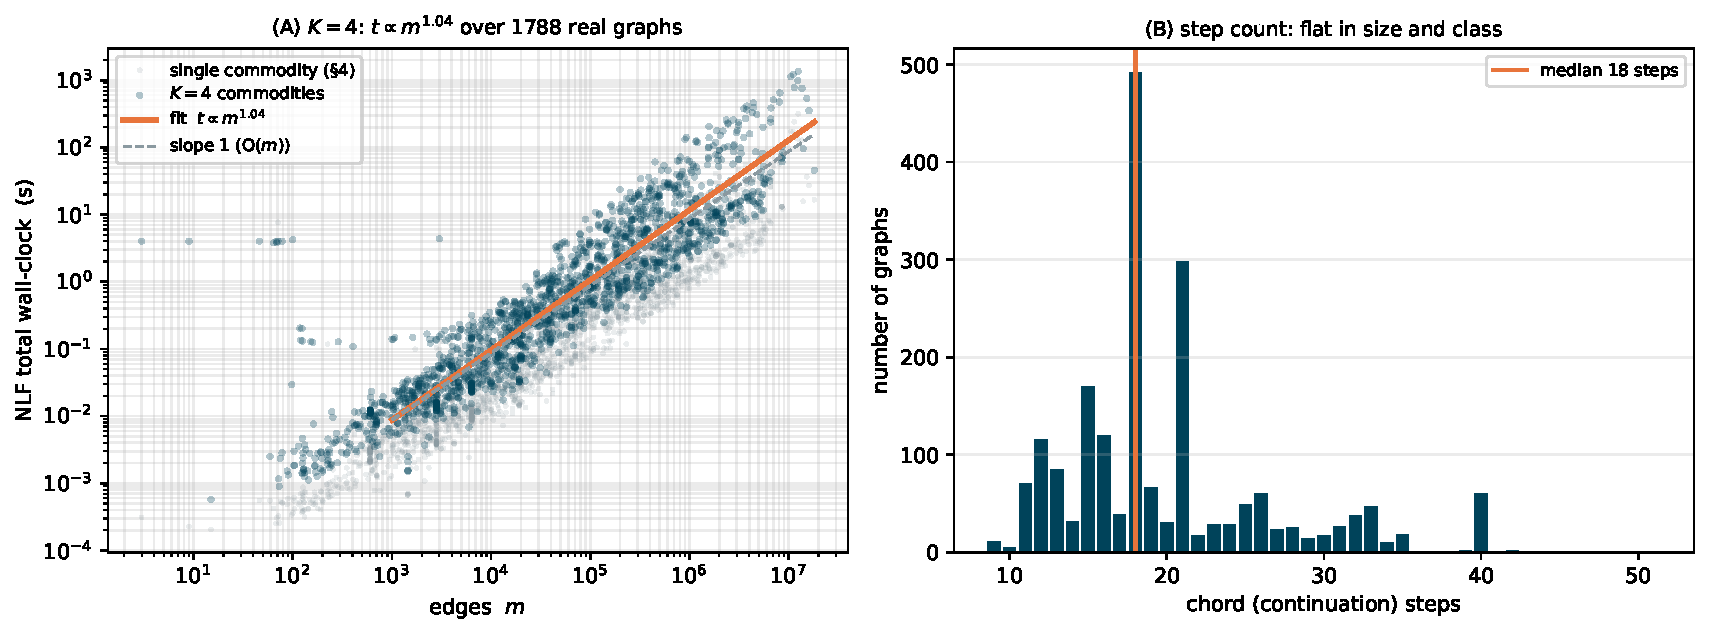
\includegraphics[width=\textwidth]{nlf_mc_corpus.pdf}
\caption{Multicommodity NLF ($K=4$) over the full real-world SuiteSparse corpus, mirroring the
single-commodity sweep (grey, underneath). (A)~Total wall-clock vs.\ edge count: all $2{,}003$
graphs converge, $t\propto m^{1.04}$ over four decades. (B)~Chord-step count: flat in size and
class, median $18$---unchanged from the single-commodity solver.}\label{fig:mccorpus}
\end{figure}

The cost of $K$ is measured directly by sweeping $K\in\{1,2,4,8\}$ with nested demand sets on FEM and
road graphs to $1.5\times10^6$ edges (\texttt{olesnik0}, \texttt{srb1}, \texttt{roadNet-PA}): the
chord-step count and the hierarchy-setup count do not move, and wall-clock grows close to linearly in
$K$ ($K{=}8$ at $4.2$--$8.5\times$ the single-commodity cost)---one shared $\Om$ setup plus $K$ cycle
solves per step, $\mathcal{O}(Km)$ in total, as the construction promises.

\section{Future work}\label{sec:extensions}
Several directions follow from the framework; we outline them, are candid that none is yet a
finished method, and seal one question---the one-shot FAS cycle---with a specific negative result
(\S\ref{sec:fasfail}).

\subsection{Directed multicommodity assignment}\label{sec:multicommodity}
\S\ref{sec:mc} routes $K$ coupled commodities under a smooth magnitude coupling with signed flows;
real traffic assignment is \emph{directed} (nonnegative arc flows, costs coupling through the directed
link flow), validated against published origin--destination equilibria (Sioux Falls, Anaheim, \dots).
Two steps separate \S\ref{sec:mc} from that target: the volume coupling $\sum_k|f^k_e|$ forces a
per-edge complementarity (only commodities whose potential drop matches the common congested cost may
flow)---a free boundary of the same character as the max-flow cut, attacked by the
continuation-with-safeguard machinery of \S\ref{sec:continuation}; and scale in $K$ (thousands of
demand columns), made conceivable by the $\mathcal{O}(Km)$ per-step cost with one shared hierarchy
(\S\ref{sec:mcalg}) plus standard per-origin aggregation. Benchmarking against Frank--Wolfe and
Algorithm-B on the published equilibria is the deployable-solver milestone.

\subsection{One-shot FAS: what we tried, and why we sealed it}\label{sec:fasfail}
The methodologically pure alternative to Algorithm~\ref{alg:fixed} is a genuinely nonlinear cycle:
nonlinear relaxation on the nodal balance, the same elimination-and-aggregation hierarchy, full
nonlinear coarse equations with the fine-to-coarse $\tau$ correction~\cite{brandt-fas,brandt-guide},
the load advanced by continuation---no global linearization anywhere. We built this prototype for the
saturating law and record its failure so it need not be rediscovered. In a controlled experiment at
\emph{fixed} load $\alpha=0.6F^{*}$ (far below the fold), from the same warm start and with equal fine
relaxation, full $\tau$-corrected V-cycles on a frozen aggregation hierarchy reached the \emph{same}
residual after $20$ cycles as Gauss--Seidel--Newton relaxation alone (slightly worse on a
$16\times16$ grid): the coarse correction removed essentially none of the smooth error---it was
\emph{inert}. Two suspects were removed by experiment: staleness (a cut-aware hierarchy frozen near
$F^{*}$ converged no better than a cut-blind one frozen at $\phi=0$, and rebuilding every step did not
help) and where $\alpha$ is updated (orthogonal; \S\ref{sec:fmg}). The surviving suspect is the
inter-grid transfer of the nonlinear state---near saturation $\rho'$ varies by orders of magnitude
within an aggregate, so a caliber-1 transfer of $\phi$ misrepresents the flux from which the coarse
$\tau$ is computed---but the flux-based transfer~\cite[\S4.6]{brandt-guide} that would test it was
never completed. Two limits keep this honest: the prototype was bespoke, not the full LAMG+ machinery
rebuilt nonlinearly, and the no-fold congestion law was never FAS-tested. We do not claim one-shot FAS
is impossible---only that its coarse levels did nothing where we tested it, and the economics remove
the incentive (the frozen-linearization solver already costs $1.9$--$4.4\times$ one linear solve).

\subsection{Full multigrid: $\alpha$ at the coarsest level}\label{sec:fmg}
Brandt's nested-iteration ideal~\cite[\S5.6]{brandt-guide} would update the global scalar $\alpha$ at
the coarsest level rather than the finest, prolongating $(\phi,\alpha)$ upward with per-level
arclength finishing. A first version was $1.6$--$2.1\times$ faster on small instances but $2.2\times$
slower on a larger grid (per-level finishing dominates)---a non-uniform gain---so we keep the simple
$\Om$ finest-level architecture and leave a tuned FMG variant to future work.

\subsection{Optimal transport as a further instance}\label{sec:ot}
The same edge-separable energy expresses optimal transport in Beckmann (flow) form: minimizing a
monotone edge-separable cost subject to $Bf=\mu-\nu$ is exactly \eqref{eq:master}---the quadratic
($H^{-1}$) cost a single $\Om$ Laplacian solve, the $W_1$ limit ($p\to1$) the non-smooth saturating
member, a natural fold instance. The quadratically-regularized form, whose dual Hessian is an
active-subgraph Laplacian solved in the literature by direct factorization~\cite{essid-solomon}, is a
natural opening for the near-linear inner solve; a dedicated treatment is left to future work.

\section{Scope and anticipated questions}\label{sec:discussion}

\paragraph{Scope, honestly stated} NLF has no combinatorial competitor on convex congestion (matches
the interior-point optimum to $10^{-10}$, empirically near-linear, wins to $45\times$ on poor
separators, \S\ref{sec:traffic}); wins $2$--$52\times$ and is often the only solver to complete on
poorly-separable graph-Laplacian flow such as communication routing
(\S\ref{sec:vsdirect},\,\ref{sec:mc}); is competitive but only asymptotically faster on well-separated
meshes and roads, where direct factorization wins; returns the cut, dual, and parametric curve on
max-flow without competing on the bare value (\S\ref{sec:maxflow}); and makes no speed claim on
DC-OPF, a motivating application only (\S\ref{sec:outofscope}). The formulation \eqref{eq:master}
itself is classical; the contribution is the unification, the frozen-linearization $\Om$ solver, and
the empirical demonstration (\S\ref{sec:priorwork}).

\emph{Why only a single source--sink demand?} This feasibility study establishes the two load-bearing
claims---that the (undirected) equilibrium is exactly \eqref{eq:master}, and that an $\Om$ inner solve
makes it linear-time. The directed full origin--destination assignment is future work
(\S\ref{sec:extensions}; \S\ref{sec:mc} is the first rung); against the directed bush-based/TAPAS
solvers~\cite{bargera2002,bargera2010}, which target that directed program and not the undirected
relaxation studied here, a same-instance comparison is the clearest remaining experiment.

\emph{Reproducibility.} Every table is produced by scripts run on public benchmarks---the SuiteSparse
collection, the Transportation Networks road data~\cite{tntp}, and the MATPOWER/pglib-opf
grids~\cite{matpower}. The interior-point comparator is Ipopt~3.14.19 with the MUMPS~5.9.0 sparse
linear solver and a $120$\,s CPU budget; the BPR law is regularized to the strictly convex,
twice-differentiable form noted in \S\ref{sec:bpr}, and the random capacity/free-flow distributions
and demand-selection seeds are fixed and recorded in the released scripts. The LAMG+ linear core is
publicly available~\cite{lamgplus}; the NLF nonlinear solver, the exact instance-generation scripts,
and a reproducibility notebook---which re-runs the fold, no-fold, and competitor timings live and
checks them against these tables---are released at \url{https://github.com/orenlivne/nlf}.

\section{Conclusion}\label{sec:conclusion}
NLF is a single resistor-network framework for convex, edge-separable network-flow equilibria
$B\,\rho(B^{\top}\phi)=\alpha d$: placing the nonlinearity in the edge law lets one energy encode
problems from electrical flow to max-flow exactly, solved by a damped chord-Newton on a frozen
linearization cycled against the nonlinear residual by a lazily refreshed near-linear Laplacian solver.
Its sharpest result is on undirected convex congestion---an interior-point optimum reproduced to
$10^{-10}$ at a size-independent step count, near-linear on poorly-separable graphs where direct
factorization is superlinear. Direct methods win on well-separated graphs and combinatorial solvers on
the bare max-flow value; the directed origin--destination assignment remains future work (the
multicommodity layer is its first rung). The contribution is the unification and the demonstration that
one frozen-linearization, multigrid-inner solver handles all of it at near-linear cost.

\appendix
\section{Why each application is an instance of the framework}\label{app:instances}
Per application: equilibrium principle $\Leftrightarrow$ convex program \eqref{eq:primal}
$\Leftrightarrow$ KKT $\Leftrightarrow$ $B\rho(B^{\top}\phi)=\alpha d$.
Each instance differs only in the edge law; directed complementarity is absorbed into that law or
relaxed by the signed formulation.

\paragraph{The chain in general} Stationarity of \eqref{eq:primal} in $f_e$ gives the nonlinear
Ohm law $t_e(f_e)=(B^{\top}\phi)_e$; inversion gives $f_e=\rho_e((B^{\top}\phi)_e)$; and
Kirchhoff ($Bf=\alpha d$) yields \eqref{eq:master}. Summing along any source--sink path telescopes:
every path has marginal cost $\phi_s-\phi_t$, the scalar equilibrium cost. The signed formulation
has no inequality constraints---a smooth equation---which is why Newton with a near-linear Laplacian
solve applies with no active sets.

\paragraph{Electrical flow (linear law)} Ohm's law is linear, $f_e=g_e/r_e$; the energy is the
dissipated power and \eqref{eq:primal} is Thomson's principle (current minimizes
dissipation)~\cite{doyle-snell}. Equation \eqref{eq:master} is the ordinary weighted Laplacian
system---the framework's fixed point under linearization, and the object the inner solver
\cite{lamgplus} is built for.

\paragraph{Congestion (traffic) equilibrium} Wardrop's principle---per origin--destination pair,
path flows $h_p\ge0$ with $\sum_p h_p=d$ obeying $T_p-\pi\ge0$ and $h_p(T_p-\pi)=0$---is, by
Beckmann's theorem~\cite{beckmann}, the KKT system of $\min_h\sum_e\int_0^{f_e}t_e$: differentiating
gives $\partial F/\partial h_p=\sum_{e\in p}t_e=T_p$, and $\pi$ (the multiplier of $\sum_p h_p=d$) is
both the marginal cost of demand and the equilibrium travel time. In link variables the demand
multiplier unfolds into the node field $\phi$ ($\pi=\phi_s-\phi_t$) and the program becomes
\eqref{eq:primal} with $\Phi_e'=t_e$, the BPR latency of \S\ref{sec:traffic}. The signed relaxation
keeps the first Wardrop clause exactly (all routes at potential-drop cost $\pi$) and discards
$h_p\ge0$: an unused route may carry counterflow---the undirected scope, with per-commodity
nonnegativity the free-boundary extension of \S\ref{sec:extensions}.

\paragraph{Minimum-delay routing} M/M/1 queueing with Little's law gives the per-packet link
delay $t_e(f)=1/(c_e-f)$, and Kleinrock's independence approximation makes total delay
edge-separable~\cite{bertsekas-gallager}. Taking the delay as marginal cost,
$\Phi_e=\log\!\big(c_e/(c_e-f)\big)$, gives \eqref{eq:primal} directly; the inverse law
$\rho_e(g)=c_e-1/g$ (odd-extended) saturates at capacity with conductance
$\rho'_e=(c_e-f)^2\to0$, placing the problem in the fold class of Table~\ref{tab:instances}: the
capacity constraint $f<c_e$ is never imposed---the law cannot produce it---and the feasibility
limit, where the filling edges form a cut in the spare capacities, is the fold handled by
\S\ref{sec:continuation}.

\paragraph{Maximum flow} The LP $\max\,\alpha$ s.t.\ $Bf=\alpha d$, $|f_e|\le c_e$ has the box
constraint as its only nonsmoothness; its complementarity (an edge is either slack with zero
reduced cost or saturated on the cut) is absorbed into the smooth saturating law \eqref{eq:rho},
whose energy $\Psi_e=c_e^2\log\cosh(g/c_e)$ is quadratic for slack edges and exactly linear,
$c_e|g|$, for saturated ones. The active set is not tracked: it \emph{emerges} as the
zero-conductance set $w_e\to0$, the forming min cut, and the LP's degeneracy reappears as the one
scalar fold at $\alpha=F^{*}$ traversed by the continuation of \S\ref{sec:continuation}. At the
fold the saturated set is the exact min cut and $\phi$ steps across it (\S\ref{sec:maxflow}); no
$(1+\epsilon)$ relaxation is involved.


\begin{thebibliography}{99}
\small
\bibitem{lamg} O.~E.~Livne and A.~Brandt, \emph{Lean Algebraic Multigrid (LAMG): Fast Graph
Laplacian Linear Solver}, SIAM J.\ Sci.\ Comput.\ \textbf{34}(4), B499--B522, 2012.
\bibitem{matpower} R.~D.~Zimmerman, C.~E.~Murillo-S\'anchez, and R.~J.~Thomas, \emph{MATPOWER:
Steady-state operations, planning, and analysis tools for power systems research and education},
IEEE Trans.\ Power Syst.\ \textbf{26}(1), 12--19, 2011.
\bibitem{powermodels} C.~Coffrin, R.~Bent, K.~Sundar, Y.~Ng, and M.~Lubin, \emph{PowerModels.jl: an
open-source framework for exploring power flow formulations}, Power Systems Computation Conf.\ (PSCC),
2018.
\bibitem{arpae-go} U.S.\ DOE ARPA-E, \emph{Grid Optimization (GO) Competition}, 2019--2023;
\texttt{https://gocompetition.energy.gov}.
\bibitem{spielman-teng} D.~A.~Spielman and S.-H.~Teng, \emph{Nearly-linear time algorithms for graph
partitioning, graph sparsification, and solving linear systems}, SIAM J.\ Comput.\ \textbf{40}(4),
981--1025, 2011.
\bibitem{koutis-cmg} I.~Koutis, G.~L.~Miller, and D.~Tolliver, \emph{Combinatorial preconditioners and
multilevel solvers for problems in computer vision and image processing}, Comput.\ Vis.\ Image
Underst.\ \textbf{115}(12), 1638--1646, 2011.
\bibitem{bindel-amg-pf} K.~Lee, H.~Wang, and D.~Bindel, \emph{A nonlinear algebraic multigrid framework
for the power flow equations}, SIAM J.\ Sci.\ Comput.\ \textbf{41}(3), B812--B833, 2019.
\bibitem{lamgplus} O.~E.~Livne, \emph{LAMG+: A Robust Lean Algebraic Multigrid Solver for Graph
Laplacians}, arXiv:2606.24791, 2026; code at \url{https://github.com/orenlivne/lamgplus}.
\bibitem{beckmann} M.~Beckmann, C.~B.~McGuire, and C.~B.~Winsten, \emph{Studies in the Economics of
Transportation}, Yale Univ.\ Press, 1956 (traffic equilibrium).
\bibitem{bpr} Bureau of Public Roads, \emph{Traffic Assignment Manual}, U.S.\ Dept.\ of Commerce,
Urban Planning Division, 1964.
\bibitem{boyles-tna} S.~D.~Boyles, N.~E.~Lownes, and A.~Unnikrishnan, \emph{Transportation Network
Analysis, Volume I: Static and Dynamic Traffic Assignment}, 2nd ed., open textbook,
\texttt{sboyles.github.io/blubook.html}, 2023 (modern treatment of Beckmann--Wardrop equilibrium and
its algorithms).
\bibitem{tntp} Transportation Networks for Research Core Team, \emph{Transportation Networks for
Research}, \texttt{github.com/bstabler/TransportationNetworks} (accessed 2026).
\bibitem{frankwolfe} M.~Frank and P.~Wolfe, \emph{An algorithm for quadratic programming}, Naval Res.\
Logist.\ Quart.\ \textbf{3}(1--2), 1956.
\bibitem{ipopt} A.~W\"achter and L.~T.~Biegler, \emph{On the implementation of an interior-point
filter line-search algorithm for large-scale nonlinear programming}, Math.\ Program.\ \textbf{106}(1),
2006 (Ipopt).
\bibitem{bertsekas-gallager} D.~Bertsekas and R.~Gallager, \emph{Data Networks}, 2nd ed., Prentice
Hall, 1992 (minimum-delay routing, Kleinrock cost).
\bibitem{mendiola-te} A.~Mendiola, J.~Astorga, E.~Jacob, and M.~Higuero, \emph{A survey on the
contributions of software-defined networking to traffic engineering}, IEEE Commun.\ Surveys Tuts.\
\textbf{19}(2), 918--953, 2017 (modern survey of delay/utilization-driven routing optimization).
\bibitem{ahuja-magnanti-orlin} R.~K.~Ahuja, T.~L.~Magnanti, and J.~B.~Orlin, \emph{Network Flows:
Theory, Algorithms, and Applications}, Prentice Hall, 1993.
\bibitem{goldberg-tarjan} A.~V.~Goldberg and R.~E.~Tarjan, \emph{A new approach to the maximum-flow
problem}, J.\ ACM \textbf{35}(4), 1988 (push--relabel).
\bibitem{goldberg-tarjan-cacm} A.~V.~Goldberg and R.~E.~Tarjan, \emph{Efficient maximum flow
algorithms}, Commun.\ ACM \textbf{57}(8), 82--89, 2014 (survey).
\bibitem{chen-almost-linear} L.~Chen, R.~Kyng, Y.~P.~Liu, R.~Peng, M.~Probst~Gutenberg, and
S.~Sachdeva, \emph{Maximum flow and minimum-cost flow in almost-linear time}, Proc.\ 63rd IEEE
Symp.\ Foundations of Computer Science (FOCS), 612--623, 2022.
\bibitem{boykov-kolmogorov} Y.~Boykov and V.~Kolmogorov, \emph{An experimental comparison of
min-cut/max-flow algorithms for energy minimization in vision}, IEEE TPAMI \textbf{26}(9), 2004.
\bibitem{dimacs} D.~S.~Johnson and C.~C.~McGeoch (eds.), \emph{Network Flows and Matching: First
DIMACS Implementation Challenge}, AMS, 1993 (\texttt{genrmf}, \texttt{washington}).
\bibitem{christiano-etal} P.~Christiano, J.~A.~Kelner, A.~Madry, D.~A.~Spielman, and S.-H.~Teng,
\emph{Electrical flows, Laplacian systems, and faster approximate maximum flow}, STOC, 2011.
\bibitem{daitch-spielman} S.~I.~Daitch and D.~A.~Spielman, \emph{Faster approximate lossy generalized
flow via interior point algorithms}, STOC, 2008.
\bibitem{approxchol} R.~Kyng and S.~Sachdeva, \emph{Approximate Gaussian elimination for
Laplacians---fast, sparse, and simple}, FOCS, 2016 (\texttt{approxChol}, implemented in
\texttt{Laplacians.jl}).
\bibitem{doyle-snell} P.~G.~Doyle and J.~L.~Snell, \emph{Random Walks and Electric Networks},
Mathematical Association of America, 1984.
\bibitem{keller} H.~B.~Keller, \emph{Numerical solution of bifurcation and nonlinear eigenvalue
problems}, in \emph{Applications of Bifurcation Theory}, Academic Press, 1977 (pseudo-arclength).
\bibitem{allgower-georg} E.~L.~Allgower and K.~Georg, \emph{Introduction to Numerical Continuation
Methods}, SIAM Classics in Applied Mathematics \textbf{45}, 2003.
\bibitem{nash-mgopt} S.~G.~Nash, \emph{A multigrid approach to discretized optimization problems},
Optim.\ Methods Softw.\ \textbf{14}(1--2), 99--116, 2000.
\bibitem{gratton-rmtr} S.~Gratton, A.~Sartenaer, and Ph.~L.~Toint, \emph{Recursive trust-region
methods for multiscale nonlinear optimization}, SIAM J.\ Optim.\ \textbf{19}(1), 414--444, 2008.
\bibitem{nocedal-wright} J.~Nocedal and S.~J.~Wright, \emph{Numerical Optimization}, 2nd ed.,
Springer, 2006.
\bibitem{inexact-newton} R.~S.~Dembo, S.~C.~Eisenstat, and T.~Steihaug, \emph{Inexact Newton methods},
SIAM J.\ Numer.\ Anal.\ \textbf{19}(2), 400--408, 1982.
\bibitem{brandt-fas} A.~Brandt, \emph{Multi-level adaptive solutions to boundary-value problems},
Math.\ Comp.\ \textbf{31}(138), 1977 (Full Approximation Scheme).
\bibitem{brandt-guide} A.~Brandt and O.~E.~Livne, \emph{Multigrid Techniques: 1984 Guide with
Applications to Fluid Dynamics, Revised Edition}, SIAM, 2011 (frozen-$\tau$ \S15; discontinuities
\S4.6; global constraints/continuation \S5.6, \S8.3).
\bibitem{gks2023} Y.~Gao, R.~Kyng, and D.~A.~Spielman, \emph{Robust and practical solution of
Laplacian equations by approximate elimination}, arXiv:2303.00709, 2023.
\bibitem{napov-notay} A.~Napov and Y.~Notay, \emph{An efficient multigrid method for graph Laplacian
systems II: robust aggregation}, SIAM J.\ Sci.\ Comput.\ \textbf{39}(5), S379--S403, 2017.
\bibitem{bargera2002} H.~Bar-Gera, \emph{Origin-based algorithm for the traffic assignment problem},
Transportation Sci.\ \textbf{36}(4), 398--417, 2002.
\bibitem{bargera2010} H.~Bar-Gera, \emph{Traffic assignment by paired alternative segments (TAPAS)},
Transportation Res.\ Part B \textbf{44}(8--9), 1022--1046, 2010.
\bibitem{essid-solomon} M.~Essid and J.~Solomon, \emph{Quadratically regularized optimal transport on
graphs}, SIAM J.\ Sci.\ Comput.\ \textbf{40}(4), A1961--A1986, 2018.
\end{thebibliography}
\end{document}
